\documentclass[oneside,12pt]{VTU_sgr}

\title{\textcolor[rgb]{0.65,0.16,0}{Human Activity Recognition using HMM based Intermediate Matching Kernel by representing videos as sequence of sets of feature vectors}}

\author{by \\ 
		\vspace{4mm}\textbf{\large{\textcolor[rgb]{0.65,0.16,0}{Rupali Bhatnagar}}} \\
		\textbf{\large{\textcolor[rgb]{0.65,0.16,0}{[Roll No. 14CSE2013]}}} \\ 
		\vspace{4mm}Under the guidance of \\
		\textbf{\large{\textcolor[rgb]{0.42,0,0.5}{Dr. Veena T.}}} \\
		 \vspace{4mm}
		 \begin{figure}[!hbtp]
\centering

\includegraphics[width=40mm]{figures/NITG-Logo.jpg}
\end{figure}
} 


\collegeordept{\vspace{-3mm} \normalsize {\textbf{\textcolor[rgb]{0,0.071,0.5}{DEPARTMENT OF COMPUTER SCIENCE AND ENGINEERING}}}}
\university{\small{\textbf{\textcolor[rgb]{0,0.071,0.5}{NATIONAL INSTITUTE OF 
TECHNOLOGY GOA}}} \\
\small{\textbf{\textcolor[rgb]{0,0.071,0.5}{FARMAGUDI, PONDA, GOA-403401, 
INDIA}}}}
\renewcommand{\submittedtext}{\vspace{3mm} Dissertation submitted in partial fulfilment of the requirements\\for the award of the degree of}
\degree{\textbf{\large{\textcolor[rgb]{0,0,1}{MASTER OF TECHNOLOGY}}}  }
\degreedate{\vspace{-4mm} 
\small{\textbf{\textcolor[rgb]{0,0.071,0.5}{\today}}}}

\hbadness=10000
\hfuzz=50pt

\usepackage{glossaries}
\usepackage{makeidx}
\usepackage{amssymb}
\usepackage{amsmath}
\usepackage{rotating}
\usepackage{enumitem}
\usepackage{multirow}
\usepackage{threeparttable}
\usepackage{fancyhdr}
\usepackage{lscape,multicol,longtable}
\usepackage{subfig}
\usepackage{url}
\usepackage{balance}
\usepackage{setspace}
\usepackage{lmodern}
\usepackage{tabularx}
\usepackage{graphics}
\usepackage{footnote}
\usepackage{multirow}
\usepackage[numbers]{natbib}
\usepackage{mathtools} % Bonus
\newtheorem{theorem}{Theorem}
\usepackage{notoccite}
\usepackage{algorithm}
\usepackage[utf8]{inputenc}
\usepackage[english]{babel}
\usepackage{amsfonts}
\usepackage{amssymb}
\usepackage{makeidx}



\usepackage[noend]{algpseudocode}
\algnewcommand{\Inputs}[1]{%
  \State \textbf{Inputs:}
  \Statex \hspace*{\algorithmicindent}\parbox[t]{.8\linewidth}{\raggedright #1}
}
\algnewcommand{\Initialize}[1]{%
  \State \textbf{Initialize:}
  \Statex \hspace*{\algorithmicindent}\parbox[t]{.8\linewidth}{\raggedright #1}
}
\DeclareMathOperator*{\argmax}{arg\,max}
\captionsetup{skip=0pt}

\newcommand\Mycite[1]{%
  \cite{#1}}


\usepackage{changepage}
\newenvironment{proof}[1][Proof]{\begin{trivlist}
\item[\hskip \labelsep {\bfseries #1}]}{\end{trivlist}}
\newenvironment{example}[1][Example]{\begin{trivlist}
\item[\hskip \labelsep {\bfseries #1}]}{\end{trivlist}}
\newenvironment{remark}[1][Remark]{\begin{trivlist}
\item[\hskip \labelsep {\bfseries #1}]}{\end{trivlist}}
\makeindex
\makeglossaries

\begin{document}

\newcommand{\keywords}[1]{\par\addvspace\baselineskip
\noindent\keywordname\enspace\ignorespaces#1}

\newcommand{\up}{\ensuremath{\mathrm{\Upsilon}}}
\newcommand{\ch}{\ensuremath{\mathcal{C}}}
\newcommand{\adv}{\ensuremath{\mathcal{A}}}
\newcommand{\advi}{\ensuremath{\mathcal{A}_i}}
\newcommand{\ui}{{\ensuremath{\mathrm{U}_{i}}}}
\newcommand{\bs}{\ensuremath{\mathcal{B}}}
\newcommand{\zp}{\ensuremath{\mathbb{Z}_p^*}}
\newcommand{\fm}{\ensuremath{\mathcal{F}}}
\newcommand{\mt}[1]{$\mathtt{#1}$} 
\newcommand{\qed}{\hfill \ensuremath{\Box}}
\newcommand{\binomwo}[2]{\genfrac{}{}{0pt}{}{#1}{#2}}
%%%%%%%%%%%%%%%%%%%%%%%%%%%%%%%%%%%%%%%%%%%%%%%%%%%%%%%%%%%%%%%%%%%%%%%%%%%%%%%%%%%%%%%%%

\renewcommand\baselinestretch{1.35}
\baselineskip=18pt plus1pt
\maketitle
\setcounter{secnumdepth}{3}
\setcounter{tocdepth}{1}

\begin{romanpages}

%\documentclass[oneside,12pt]{article}
%\title{}
%%\hbadness=10000
%%\hfuzz=50pt
%
%\usepackage{graphicx}
%\pagenumbering{gobble}
%\begin{document}
%
%

\begin{center}

\setlength{\headheight}{0pt}

Department of Computer Science and Engineering \\
National Institute Of Technology,Goa \\
Farmagudi, Ponda $403 401$, Goa, India
\end{center}
\vspace{10mm}
\begin{center}
\begin{Huge}
\textbf{CERTIFICATE}
\end{Huge}


					\begin{figure}[h]
					\begin{center}
					
\includegraphics[width=40mm]{figures/NITG-Logo.jpg}
					\end{center}
					\end{figure}
\end{center}
\vspace{6mm}

\begin{large}
\noindent{
This is to	certify that the Major Project Report titled \textbf{``Human Activity Recognition using HMM based Intermediate Matching Kernel by representing videos as sequence of sets of feature vectors"} submitted by \textbf{Rupali Bhatnagar} bearing \textbf{Roll No. 14CSE2013} to National Institute of Technology Goa towards partial fulfilment of Matster of Technology in Computer Science and Engineering is a bona fide record of the work  carried out by him under my supervision.}


\vspace{10mm}


\begin{flushleft}
\textsc{Date} \hfill \textsc{Supervisor}
\vspace{4mm}


\textsc{Place} \hfill \textsc{Head of the Department}\\
\textsc{} \hfill Department of CSE \\
\textsc{} \hfill NIT Goa

\end{flushleft}


\end{large}

%\end{document}


%\pdfbookmark{Acknowledgement}{Acknowledgement}
%\begin{acknowledgments}
\setlength{\parskip}{10pt plus 5pt minus 3pt}
\setlength{\parindent}{20pt}%



\end{acknowledgments}
% ------------------------------------------------------------------------


\chapter*{Dedication}
\addcontentsline{toc}{chapter}{Dedication}

% Add your dedication text here.

\clearpage


\pdfbookmark{Abstract}{Abstract}
\begin{abstracts}  
\normalsize
\setlength{\parskip}{10pt plus 5pt minus 3pt}
\setlength{\parindent}{20pt}%
%\fontsize{12pt}{12pt}\selectionfont

Human activity recognition is the task of classifying a sequence of human actions. The task of human activity recognition is manifold: first task is to identify the time interval where activity has taken place and then to classify the activity based on the composing actions. 

Videos provide a time-ordering of a set of related frames where each frame is composed of pixels.The video,then can be visualized as 3D matrix of pixels wherein the first two dimensions of the matrix provide for spatial data and the third dimension refers to time.

The spatial patterns observed in the video correspond to the presence of objects,
backgrounds, textures and other interest points. The temporal patterns on the other hand capture the motion of these observed objects or regions of interest. Both these factors are important for deciding the activity class of a video.

Our proposed approach represents the video as a sequence of feature vectors which capture the spatial and temporal information. Each video is represented a set of frame feature vectors. The representation of each video then depends on the duration of the video. This results in variable length feature vector representation for each video.For the classifier, we propose to use kernel based SVM in which the kernel is a dynamic kernel. The kernel that we propose to use is the HMM based Intermediate Matching Kernel since it is capable of modeling the sequential information modeled in the videos.
\end{abstracts}

% ----------------------------------------------------------------------




\pdfbookmark[0]{Content}{content}
\fancyhead[LE]{\bfseries\small{Contents}}
\fancyhead[RO]{\bfseries\small{Contents}} \tableofcontents
\clearpage \pdfbookmark[1]{List of Figures}{lof}
\fancyhead[LE]{\bfseries\small{List of Figures}}
\fancyhead[RO]{\bfseries\small{List of Figures}} \listoffigures
\clearpage
\pdfbookmark[1]{List of Tables}{lot}
\fancyhead[LE]{\bfseries\small{List of Tables}}
\fancyhead[RO]{\bfseries\small{List of Tables}} \listoftables 

\clearpage

\phantomsection

\pdfbookmark[1]{List of Abbreviations}{loa}
\newglossaryentry{HoG}{name={HoG},
description={histogram of oriented gradients}}
\end{romanpages}


\fancyhf{} \fancyhead[LE]{\bfseries\small{\leftmark}}
\fancyhead[RO]{\bfseries\small{\rightmark}}
\fancyfoot[CE,CO]{\bfseries\thepage} \setcounter{page}{1}
\pagenumbering{arabic}
\renewcommand{\labelenumi}{(\roman{enumi})}  


\chapter{Introduction}\label{Introduction}
\thispagestyle{empty}
\setlength{\parskip}{10pt plus 5pt minus 3pt}
\setlength{\parindent}{20pt}%

Human activity recognition can be defined as the task of identifying a sequence of actions and classifying them into various classes. Human activity recognition is an important area of computer vision and has found applications in various fields like 
surveillance systems, video retrieval systems, patient monitoring systems, predicting crowd behavior, etc.The task of human activity recognition consists of the following steps:\begin{enumerate}
\item Getting the low level representation from videos
\item Using the low level representation to get features that better describe the video
\item Using the features extracted above to classify the videos into the predefined classes
\end{enumerate}

Videos contain massive amount of information in the terms of spatio-temporal pixel  intensity variations.\Mycite{MRSurvey} Extracting both the spatial information as well as the temporal information is necessary for the task of video classification. The spatial information identifies the appearance based information like, objects, gradients, backgrounds etc from the video while the temporal information helps to identify the motion between the identified appearance based features.

The task of video classification however becomes complex due to the limitations inherent in the data. The following challenges are faced in the task:-
\begin{enumerate}
\item Varying length representations-
A video's inherent attribute is it's duration or length. The length of the video
affects the number of frames present in it. The more the length of the video, more are the number of frames associated with it. Therefore, when we map features from the video data,we get a varying length feature for each video.

\item High Dimensionality-
The image data has very high dimensionality due to the spatial information
captured by it's pixels. Drawing inferences from data of such high dimensions
soon becomes intractable. We know that videos are sequence of images. So
in case of images, only spatial modeling is required, but we need to represent
temporal information also when dealing with videos.

\item Intra-class variability-
Within video belonging to the same class, there is a lot of variation in terms
of appearance, color and duration of the video.This results in a high intra-class
variability due to which efficient representations are difficult to implement.

\item Inter-class similarity-
The video belonging to different classes may have many things in common, for
example, background, objects, etc.

\item Action vocabulary is not well defined-
Various actions and activities are not well defined, for example, opening an umbrella, closing a door, closing a faucet,etc

\end{enumerate}

\section{Problem Definition}
It is easy to note from the above section that the task of human activity recognition is a complex task which has lot of scope in the real world applications. The task of classification then requires us to choose a suitable feature representation and classification strategy to efficiently capture and utilize appearance based and motion based information from the videos.\\

Videos are a collection of spatially and temporally related frames. To capture the spatial as well as temporal information, we need to define features that inter-class similarities and intra-class variations.\\

Since the feature representation for each video would be dependent on the number of frames it possesses, we need to define a classifier that takes into consideration the varying length representation of the videos.\\

This report is arranged as follows: we discuss the related work in Chapter \ref{Related_Work}. We then discuss the features that may be extracted from the videos in Chapter \ref{Feature_Extraction}. We look at the various classifiers and discuss their advantages and disadvantages in Chapter \ref{Classifiers}. We then present our model in Chapter \ref{Proposed_Approach}. Chapter \ref{Observations} and Chapter \ref{Conclusion} presents the experimental works and conclusions.
\chapter{Related Work}\label{Related_Work}
\thispagestyle{empty}
\setlength{\parskip}{10pt plus 5pt minus 3pt}
\setlength{\parindent}{20pt}%

In literature, we find a number of video classification strategies, each having its benefits and limitations. In this chapter we learn about the various methodologies that have been put into use for classifying videos.

\section{Gaussian Mixture Models}
Gaussian Mixture Model is a generative model for pattern recognition where it extends the basic Gaussian model to contain $k_i$ components for Class $i$. With each component is associated a different set of parameters which need to be learned separately.
\begin{enumerate}
\item Gaussian mixture models (GMMs) as used by \citet{GMM} are commonly used for classification of varying length patterns represented as sets of feature vectors. Maximum likelihood (ML) based method is commonly used for estimation of parameters of a GMM for each class, when sufficient training data is available.When the training data available for a class is limited, robust estimates of parameters can be obtained through maximum a posteriori (MAP) adaptation of a class-independent GMM (CIGMM) to the training data of each class.

\item In another methodology proposed in \citet{PCA_GMM}, the authors use statistical signal modeling approach and the PCA for the purpose of video classification using GMM. The audio and video features are taken in conjunction to form a `super' vector whose dimensionality is reduced using PCA. Then using Expectation Maximization algorithm for GMM, they model the features for the different genres.
\begin{figure}[!hbtp]
\centering
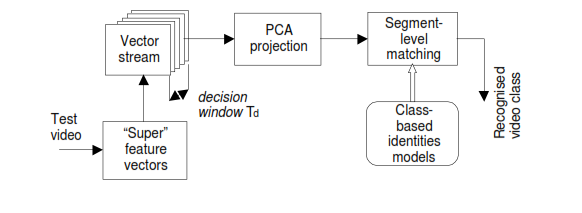
\includegraphics[scale=1]{figures/Chapter3/PCA_GMM.png}
\caption{Temporal Video Genre Classification using \cite{PCA_GMM} approach}
\end{figure}

\end{enumerate}

\section{Hidden Markov Models (HMM)}
The Hidden Markov model (HMM) is widely used for classifying sequential data. An HMM represents a set of states and the probabilities of making a transition from one state to another state.The typical usage in video classification is to train one HMM for each class. When presented with a test sequence of features, the sequence will be assigned to the class whose HMM can reproduce the sequence with the highest probability.\cite{Survey}

\begin{enumerate}
\item In \citet{CMLT}, a temporal kernel called Correlative Multilabel Temporal(CMLT) Kernel is introduced using correlative multi-label formulation which can leverage the concept interactions as well as low-level feature dynamics to boost the video event detection. It first adapts a universal reference model (URM) to a HMM for an individual video sequences.Then similarities can then be computed between these HMMs as temporal kernel based on their discrimination distances.


 
\item In the model proposed by \citet{Active} called Activity Concept Transitions in Video Events(ACTIVE), a video event is a sequence of activity concepts. A new concept is generated with certain probabilities based on the previous concept. An observation is a low level feature vector from a sub-clip and generated based on the concepts. Then the feature vector is obtained by using Fisher Kernel over the HMM. The features are then classifies using an SVM.

\end{enumerate}

\section{SVM}
SVM is one of the best and most widely used classifiers. Many classification algorithms use SVM as the main classifier after the feature selection procedure. This is primarily because SVM has a good generalization capability. We now discuss a few SVM based approaches present in literature.
\begin{enumerate}

\item \citet{Yegna} do video classification based on color, shape and motion features using support vector machine models. They use 3 types of features:-
\begin{itemize}
\item Color Features which include 3 moments of color histograms- mean, variance and skewness
\item Shape features that use edge histograms
\item Motion features where  motion is extracted by pixel-wise differencing of consecutive frames.

\end{itemize} Then using one-versus-rest approach, they use these feature vectors for SVM classification.

\item A  modified Directed Acyclic Graph Support Vector Machine (DAGSVM) model has been presented by \citet{DAGSVM} in which they have used features of editing, color,texture and motion form the video. Then, they have used one-to-one SVM that has been arranged as Directed Acyclic Graph because it yields faster performance.
\begin{figure}[!hbtp]
\centering
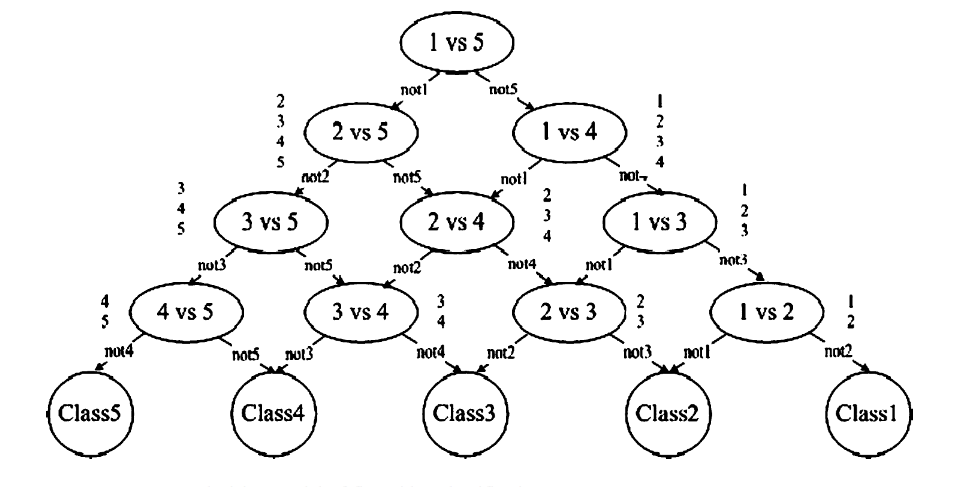
\includegraphics[scale=0.5]{figures/Chapter3/DAGSVM.png}
\caption{DAGSVM for Video Classification by \citet{DAGSVM}}
\end{figure}

\item \citet{Hierarchical_SVM} proposed an Hierarchical SVM scheme that uses ten computable spatio-temporal features to distinguish the different genres This model consists of a series of SVM classifiers united in a binary-tree form.  This scheme used 2 types of features:
\begin{itemize}
\item Temporal Features  which include average shot length, cut percentage, average color difference and camera motion. 
\item Spatial Features which include face frames ratio, average brightness and average color entropy.
\end{itemize} 
\begin{figure}[!hbtp]
\centering
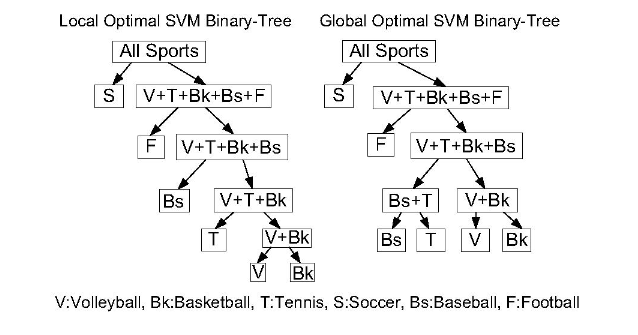
\includegraphics[scale=0.9]{figures/Chapter3/Hierarchical_SVM.png}
\caption{Local and Global optimal SVM Binary Tree by \citet{Hierarchical_SVM}}
\end{figure}
\newpage
Using these features, the proposed method creates 2 types of trees:-
\begin{itemize}
\item A local optimal SVM binary tree that attempts to find the best separation at each node using 2-fold cross-validation. which aims at finding the best separation at each node locally.
\item A global optimal SVM tree performs a global optimization of the SVM binary tree by performing the cross-validation for each possible binary tree and rhen choosing the one with the highest accuracy.
\end{itemize} 

\item In the method proposed by \citet{String_kernel}, events are modeled as a sequence composed of histograms of visual features, computed from each frame using the traditional BoW. The sequences are
treated as strings (phrases) where each histogram is considered as a character. Event
classification of these sequences of variable length, depending on the duration ofthe video clips, are performed using SVM classifiers with a string kernel that usesthe Needlemann-Wunsch edit distance. The basic idea of the algorithm is to build up the best alignment through optimal alignments of smaller subsequences, using dynamic programming,unlike other approaches, such as dynamic time warping. The proposed kernel is of the form- $ K(x,x')=\exp{(-d(x,x'))}$ where $ d(x,x') $ is the Needleman-Wunsch edit distance between $x$ and $x'$.

\begin{figure}[!hbtp]
\centering
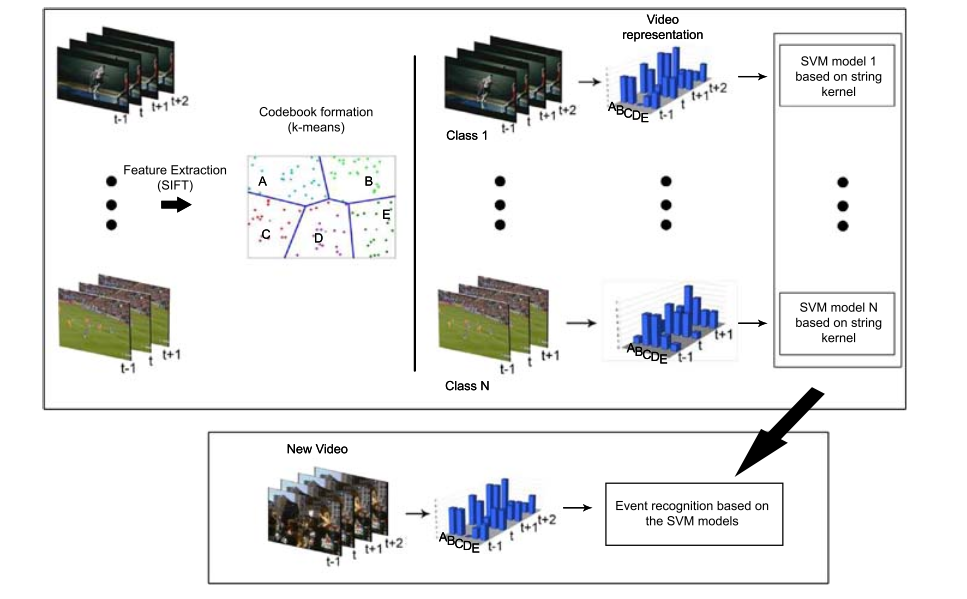
\includegraphics[scale=0.6]{figures/Chapter3/String_kernel.png}
\caption{String Kernel approach of \citet{String_kernel}}
\end{figure}


\item \citet{Motion_Words} propose the use of Motion Words for Videos for video classification.They pool features over supervoxelsby segmenting the video into supervoxels,using video segmentation . The proposed representation enables
localization of common regions across videos in both space and time that yields meaningful regions, resulting in interpretative features.

\begin{figure}[!hbtp]
 \centering
 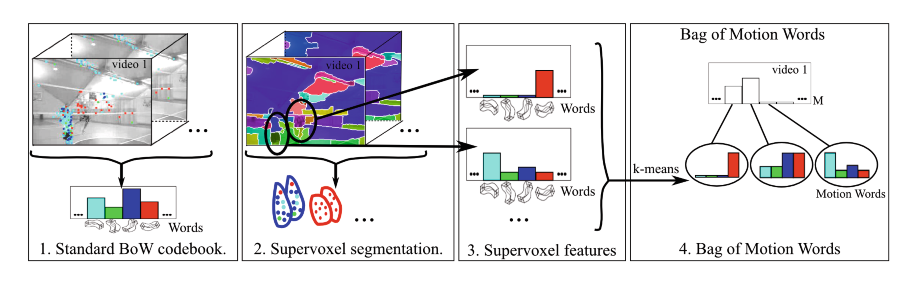
\includegraphics[scale=0.7]{figures/Chapter3/Motion_Words.png}
 \caption{Bag of Motion Words method by \citet{Motion_Words}}
 \end{figure}


For constructing the Bag of Motion Words, 
\begin{itemize}
\item Compute a standard Bag of Words code-book from low-level descriptors
\item Compute a supervoxel segmentation
\item Pool the encoded low-level descriptors in each supervoxel to obtain
supervoxel-based feature vectors
\item Cluster the supervoxel-based vectors to learn a code-book of Motion Words.
\end{itemize}  


\item \citet{Feature_Kernel} have proposed a kernel for matching feature sequences
based on the LCSS distance measure and integrating the MPEG-7 kernel. They use 4 MPEG-7 features- Color Layout (CLD), Dominant Color (DCD), Color Structure (CSD) and Edge Histogram (EHD). The joint kernel is of the form-
\begin{equation}
K_{mpeg-7}(x,x')=\Pi_{i=cld,dcd,csd,ehd} \exp{(-w_i K_i(x,x'))}
\end{equation}
where $K_i(x,x')$ is the specific kernel for each feature.Apart from kernel based on features, they have also used a kernel based on the distance of subsequences of feature vectors in order to deal with sequences of feature vectors. For this they use a kernel that is based on the \textit{longest common subsequence kernel}.


\item For the purpose of video classification,\citet{DACO} represent actions directlyas time series of frames and propose to model the event's key dynamic aspects by using auto-correlation.That is they use the cross-correlation of the signal of frames with a temporally shifted version of itself, defined as the distance measure \textit{Hilbert-Schmidt norm} of the difference between auto-correlations. The associated Gaussian RBF kernel is called the Difference between Auto-Correlation Operators (DACO) kernel. The motivation behind the DACO kernel is that the distance will tend to be smaller for time series with almost no temporal structure (e.g. for random sequences of frames) and bigger for actions with quasi-deterministic relationships between neighboring frames (e.g. a constant translation movement). 



\item Multiple kernel learning (MKL) has been proposed by \citet{MKL} for problems, where instead of choosing a kernel a priori, weights for combining different kernels are learned together with the model. Multiple kernel learning (MKL) is an approach that considers
a set of kernels potentially appropriate for their problems, and estimates both the parameters of the individual kernels as well as their relative weights during the training
phase. The weights are assigned using the interleaved optimization method.

\item \citet{Online_Concept} proposed sliding window variants of three approaches for sequence-based kernels -temporal pyramid matching, all subsequences, longest common subsequence and show how they can be efficiently applied to online concept detection by use of sliding window segmentation.
 \end{enumerate}

%\bibliographystyle{ieeetr} 
%\bibliography{biblio}
%\end{document}
\chapter{Feature Extraction}\label{Feature_Extraction}
\thispagestyle{empty}
\setlength{\parskip}{10pt plus 5pt minus 3pt}
\setlength{\parindent}{20pt}%

There are various kinds of descriptors which can be broadly divided into 2:-
\begin{enumerate}
\item Global Descriptors - They are sensitive to noise, occlusion and viewpoint variations.
\item Local Descriptors - These are low level descriptors which include the following:-
	\begin{enumerate}
		\item Image descriptors - These lack any kind of time information.
 				Example-SIFT, HOG , Harris.
 		\item Space-time descriptors - They preserve temporal information while extracting the local features. Some of them are the temporal extension of image descriptors. Example-3D-SIFT,HOG3D,spatio-temporal Harris interest points. While others capture the video information directly like MIP,HOG-HOF,SCISA,etc.
 \end{enumerate}
 \end{enumerate}
After extracting the descriptors, use of holistic encoding techniques like BoF and FV is done to derive a vector for each video sequence.

\section{Feature Descriptors}
The hand crafted features for video data basically compose of 3 categories of features:-
\begin{itemize}
\item Appearance based features that rely on color-based features, edge \& shape based features.
\item Motion based features estimated features using motion information that is embedded in the system.
\item Audio based features use audio information that is present within the video.
\end{itemize}
\subsection{Appearance Based Features}
In this we discuss the 3 most commonly used features, that are, Histogram of oriented gradients(HoG), Space Invariant Feature Transforms(SIFT) \& Speeded-Up Robust Features(SURF).
\subsubsection{Histogram of Oriented gradients (HOG)}
The histogram of oriented gradients(HOG) \Mycite{HOG} is a feature descriptor used for the purpose of object detection. Intuitively it tries to capture the shape of structures in the region by capturing information about gradients. It does so by dividing the image into small (usually 8x8 pixels) cells and blocks of 4x4 cells. Each cell has a fixed number of gradient orientation bins. Each pixel in the cell votes for a gradient orientation bin with a vote proportional to the gradient magnitude at that pixel.

To reduce aliasing, the pixels votes are bilinearly interpolated. This interpolation happens in both the orientation as position. This statement is important - it means that a pixel will not only vote for its orientation bin, but also for the neighboring orientation bins  Similarly, it will vote for these two orientation bins not only in its cell, but also in the 4 neighboring cells of its cell. The weights here are decided by the distance of the pixel from the cell centers.

Histograms are also normalized based on their energy (regularized L2 norm) across blocks. Since the blocks have a step size of 1 cell, a cell will be part of 4 blocks. This defines four differently normalized versions of the cell's histogram. These 4 histograms are concatenated to get the descriptor for the cell. 
\begin{figure}[!hbtp]
\centering
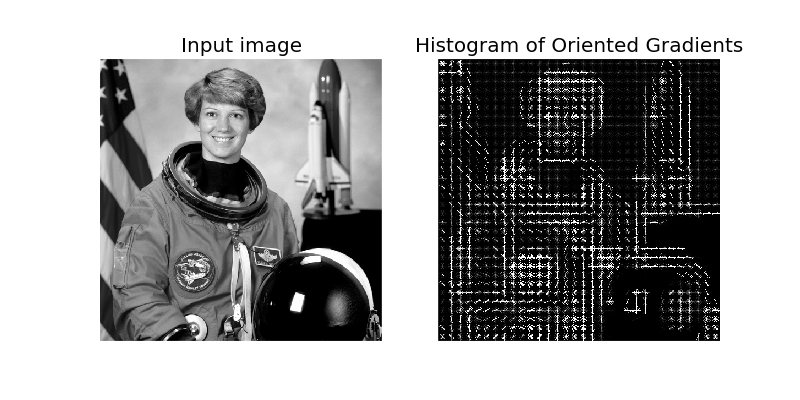
\includegraphics[scale=0.5]{figures/Chapter4/HOG2.png}
\caption{Example of Histogram of Oriented Gradients \Mycite{HOG}}
\end{figure}



\subsubsection{Scale Invariant Feature Transform(SIFT)}
In Harris Corner detection,the features are rotation-invariant but not scale invariant.So, in \citet{SIFT} proposed an algorithm which extracts keypoints and compute its descriptors. There are mainly four steps involved in SIFT algorithm. 
\begin{enumerate}
\item Scale-space extrema detection: The first stage of computation searches over all scales and image locations. It is implemented efficiently by using a difference-of-Gaussian
function to identify potential interest points that are invariant to scale and orientation.
\begin{figure}[!hbtp]
\centering
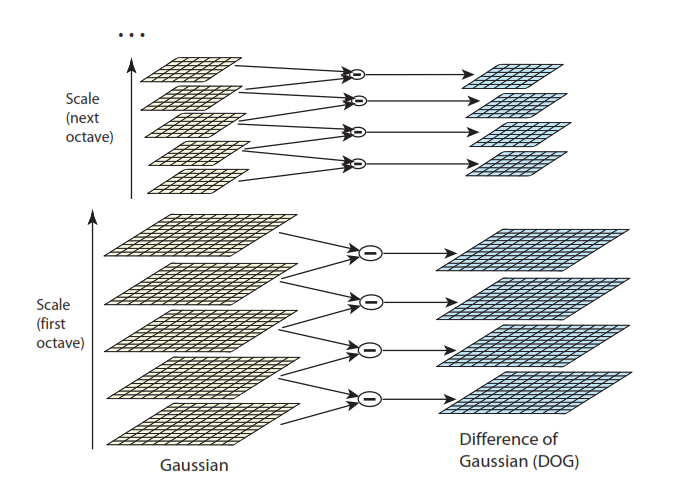
\includegraphics[scale=0.8]{figures/Chapter4/SIFT1.png}
\caption{Difference of Gaussians for SIFT \Mycite{SIFT}}
\end{figure}

\item Keypoint localization: At each candidate location, a detailed model is fit to determine location and scale. Keypoints are selected based on measures of their stability.

\item Orientation assignment: One or more orientations are assigned to each keypoint location based on local image gradient directions. All future operations are performed
on image data that has been transformed relative to the assigned orientation, scale, and
location for each feature, thereby providing invariance to these transformations.

\begin{figure}[!hbtp]
\centering
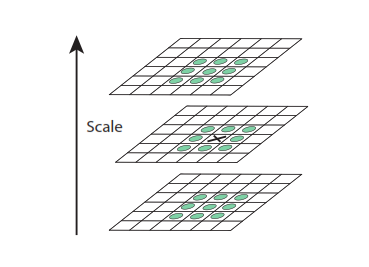
\includegraphics[scale=1]{figures/Chapter4/SIFT2.png}
\caption{Keypoint Localization in SIFT \Mycite{SIFT}}
\end{figure}

\item Keypoint descriptor: The local image gradients are measured at the selected scale
in the region around each keypoint. These are transformed into a representation that
allows for significant levels of local shape distortion and change in illumination
\end{enumerate}
\begin{figure}[!hbtp]
\centering
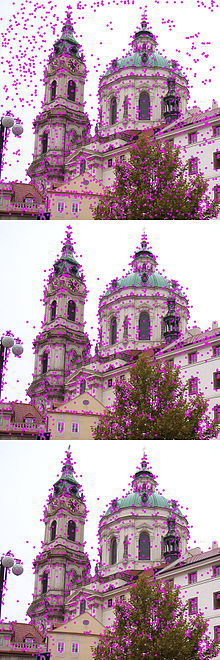
\includegraphics[scale=0.5]{figures/Chapter4/SIFT3.jpg}
\caption{Example of SIFT\Mycite{book_SIFT}}
\end{figure}
\newpage
\subsubsection{Speeded-Up Robust Features(SURF)}
In SIFT, Lowe approximated Laplacian of Gaussian with Difference of Gaussian for finding scale-space. SURF goes a little further and approximates LoG with Box Filter. One big advantage of this approximation is that, convolution with box filter can be easily calculated with the help of integral images. And it can be done in parallel for different scales. Also the SURF rely on determinant of Hessian matrix for both scale and location.\\
\begin{figure}[!hbtp]
\centering
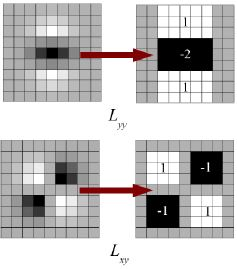
\includegraphics[scale=0.5]{figures/Chapter4/SURF1.jpg}
\caption{Approximation of LoG in SURF\Mycite{SURF}}
\end{figure}
\\
For orientation assignment, SURF uses wavelet responses in horizontal and vertical direction for a neighborhood of size 6s. Adequate Guassian weights are also applied to it.  The dominant orientation is estimated by calculating the sum of all responses within a sliding orientation window of angle 60 degrees. Interesting thing is that, wavelet response can be found out using integral images very easily at any scale. For many applications, rotation invariance is not required, so no need of finding this orientation, which speeds up the process. SURF provides such a functionality called Upright-SURF or U-SURF. It improves speed and is robust upto $\pm 15^{\circ}$.If it is 0, orientation is calculated. If it is 1, orientation is not calculated and it is more faster.
\begin{figure}[!hbtp]
\centering
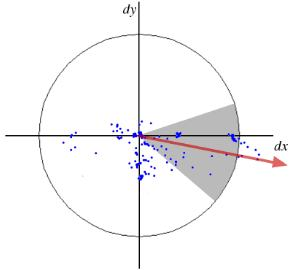
\includegraphics[scale=0.5]{figures/Chapter4/SURF2.jpg}
\caption{Plotting of wavelet responses in SURF\Mycite{SURF}}
\end{figure}\\
For feature description, SURF uses Wavelet responses in horizontal and vertical direction (again, use of integral images makes things easier). A neighbourhood of size 20sX20s is taken around the keypoint where s is the size. It is divided into 4x4 subregions. For each subregion, horizontal and vertical wavelet responses are taken and a vector is formed like this, v=$( \sum{d_x}, \sum{d_y}, \sum{|d_x|}, \sum{|d_y|})$. This when represented as a vector gives SURF feature descriptor with total 64 dimensions. Lower the dimension, higher the speed of computation and matching, but provide better distinctiveness of features.

For more distinctiveness, SURF feature descriptor has an extended 128 dimension version. The sums of $d_x$ and $|d_x|$ are computed separately for $d_y < 0$ and $d_y \geq 0$. Similarly, the sums of $d_y$ and $|d_y|$ are split up according to the sign of $d_x$ , thereby doubling the number of features. It doesn’t add much computation complexity. 

Another important improvement is the use of sign of Laplacian (trace of Hessian Matrix) for underlying interest point. It adds no computation cost since it is already computed during detection. The sign of the Laplacian distinguishes bright blobs on dark backgrounds from the reverse situation. In the matching stage, we only compare features if they have the same type of contrast. This minimal information allows for faster matching, without reducing the descriptor’s performance.\\
\begin{figure}[!hbtp]
\centering
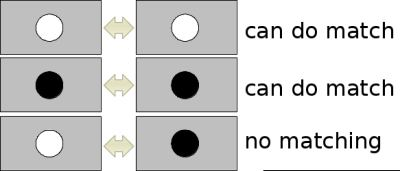
\includegraphics[scale=0.5]{figures/Chapter4/SURF3.jpg}
\caption{Comparing of features in SURF\Mycite{SURF}}
\end{figure}




\subsection{Motion Based Features}

\subsubsection{Space Time Interest Points(STIP)}
To detect spatio-temporal events, STIP builds on the idea of the Harris and Forstner interest point operators and detects local structures in space-time where the image values have significant local variations in both space and time.Then, the spatio-temporal extents of the detected events are estimated and their scale-invariant spatio-temporal descriptors are computed.Using such descriptors, they classify events and construct video representation in terms of labeled space-time points.\Mycite{STIP}In this case:

\begin{itemize}
\item Videos are considered as volumes of pixels.
\item Spatio-temporal features are located at spatio-temporal salient points that are extracted with interest point operators.
\item Interest point structures are searched for that are stable under  rotation, viewpoint, scale and illumination changes.
\end{itemize} 

So, space time interest point detectors are extensions of 2D interest point detectors that incorporate temporal information.They are based on the detection of spatio-temporal corners which are located in region that exhibits a high variation of image intensity in all
three directions $(x, y,t)$. This requires that spatio-temporal corners are located at spatial corners such that they invert motion in two consecutive frames (high temporal gradient variation). They are identified from local maxima of a cornerness function computed for all pixels across spatial and temporal scales.
\\
\begin{figure}[!hbtp]
\centering
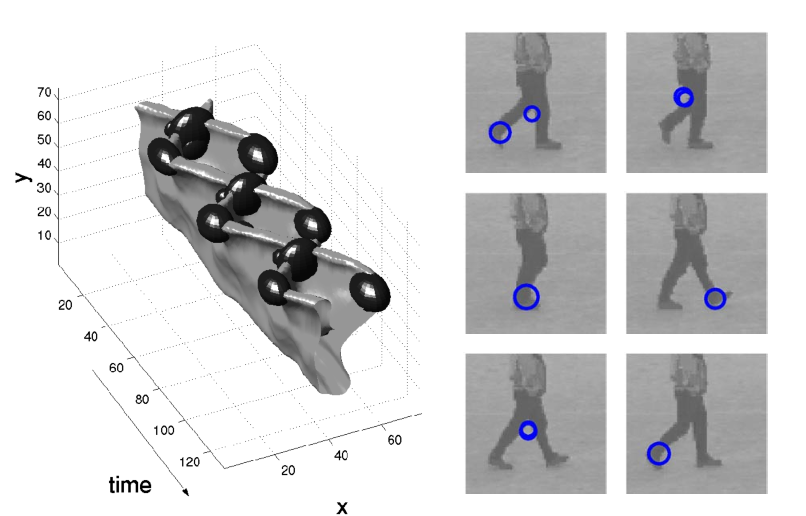
\includegraphics[scale=0.5]{figures/Chapter4/STIP.png}
\caption{Example of STIP \Mycite{STIP}}
\end{figure}
\\
\subsubsection{Optical Flow}
Optical flow is the pattern of apparent motion of image objects between two consecutive frames caused by the movement of object or camera. It is 2D vector field where each vector is a displacement vector showing the movement of points from first frame to second.\Mycite{Optical_flow}
Optical flow works on several assumptions:
\begin{itemize}
\item The pixel intensities of an object do not change between consecutive frames.
\item Neighboring pixels have similar motion. 
\end{itemize}
Consider a pixel $I(x,y,t)$ in first frame. It moves by distance $(dx,dy)$ in next frame taken after $dt$ time. So since those pixels are the same and intensity does not change, we can say,
\begin{equation}
I(x,y,t) = I(x+dx, y+dy, t+dt)
\end{equation}
Then take Taylor series approximation of right-hand side, remove common terms and divide by $dt$ to get the following equation:
\begin{equation}
f_x u + f_y v + f_t = 0 
\end{equation}
where
\begin{equation}
f_x = \frac{\partial f}{\partial x} \quad
f_y = \frac{\partial f}{\partial x} \quad
u = \frac{dx}{dt} \quad
v = \frac{dy}{dt}
\end{equation}
Above equation is called Optical Flow equation. In it, we can find $f_x$ and $f_y$, they are image gradients. Similarly $f_t$ is the gradient along time. But $(u,v)$ is unknown. We cannot solve this one equation with two unknown variables. So several methods are provided to solve this problem and one of them is Lucas-Kanade.

\textbf{Lucas Kanade method}-\\
We have seen an assumption before, that all the neighboring pixels will have similar motion. Lucas-Kanade method takes a $3x3$ patch around the point. So all the 9 points have the same motion. We can find $(f_x, f_y, f_t)$ for these 9 points. So now our problem becomes solving 9 equations with two unknown variables which is over-determined. A better solution is obtained with least square fit method. Below is the final solution which is two equation-two unknown problem and solve to get the solution.
\begin{equation}
\begin{bmatrix} u \\ v \end{bmatrix} =
\begin{bmatrix}
    \sum_{i}{f_{x_i}}^2  &  \sum_{i}{f_{x_i} f_{y_i} } \\
    \sum_{i}{f_{x_i} f_{y_i}} & \sum_{i}{f_{y_i}}^2
\end{bmatrix}^{-1}
\begin{bmatrix}
    - \sum_{i}{f_{x_i} f_{t_i}} \\
    - \sum_{i}{f_{y_i} f_{t_i}}
\end{bmatrix}
\end{equation}
So from user point of view, idea is simple, we give some points to track, we receive the optical flow vectors of those points. But again there are some problems. Until now, we were dealing with small motions. So it fails when there is large motion. So again we go for pyramids. When we go up in the pyramid, small motions are removed and large motions becomes small motions. So applying Lucas-Kanade there, we get optical flow along with the scale.

\subsubsection{Improved Trajectories}
These extracted trajectories are mainly located at regions with high motion salience, which contain rich and discriminative information. These local descriptors of the corresponding regions in several successive frames, are aligned and pooled along the trajectories. This trajectory constrained sampling strategy also takes account of the temporal continuity of human action, and is effective to deal with the variations of motion speed. However, these hand-crafted descriptors are not optimized for visual representation and may lack discriminative capacity for action recognition. To compute dense trajectories, 
\begin{enumerate}
\item  Densely sample a set of points on 8 spatial scales on a grid with step size of 5 pixels. Points in homogeneous areas are eliminated by setting a threshold for the smaller eigenvalue of their auto-correlation matrices. Then these sampled points
are tracked by media filtering of dense flow field.
\item The static trajectories are removed as they lack motion information, and other trajectories with suddenly large displacement are also ignored, since they are obviously incorrect due to inaccurate optical flow.
\end{enumerate}

\subsection{Audio Features}
Audio features can lead to three layers of audio understanding\Mycite{Survey} : Low-level acoustics, such as the average frequency for a frame, Mid-level sound objects, such as the audio signature of the sound a ball makes while bouncing, and High-level scene classes, such as background music playing in certain types of video scenes.

Audio features can be derived from either the time domain or the frequency domain. 
\begin{enumerate}
\item Time Domain Features-\\
The root mean square (RMS) of the signal energy approximates the human perception of
the loudness or volume of a sound .

\begin{itemize}
\item Zero crossing rate (ZCR) is the number of signal amplitude sign changes in the current frame. Higher frequencies result in higher zero crossing rates. Speech normally has a higher variability of the ZCR than in music. If the loudness and ZCR are both below thresholds, then this frame may represent silence.
\item The silence ratio is the proportion of a frame with amplitude values below some threshold. Speech normally has a higher silence ratio than music. 
\end{itemize}

\item Frequency Domain Features-\\
The energy distribution is the signal distribution across frequency components. 
\begin{itemize}
\item Brightness is approximated by the frequency centroid, provides a measure of where the frequency components are concentrated. Brightness is higher for music than speech.
\item Bandwidth is the measure of frequency range of the signal.
\item The fundamental frequency is the lowest frequency in a sample and approximates pitch, which is a subjective measure.
\item Mel-frequency cepstral coefficients (MFCC) are produced by taking the logarithm of the spectral components and then placing them into bins based upon the Mel frequency scale,
which is perception-based. This is followed by applying the discrete cosine transform (DCT)

\end{itemize}
\end{enumerate}


\section{Feature Encoding Methods}
There are 2 feature encoding methods when we consider a holistic approach:-
\begin{enumerate}
	\item Bag of Features - It is a standard approach in which we quantize the features into a predefined codebook.It is an orderless document representation methodology in which we compute the feature descriptors , then cluster them to get a frequency representation by use of hard clustering like KNN clustering. The mechanism is shown in Figure \ref{Bow}.
		
	\begin{figure}[hbtp]
	\centering
	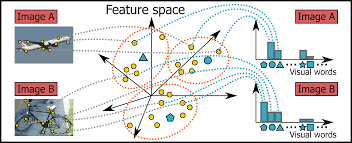
\includegraphics[scale=0.5]{figures/Feature_extraction/BoW.png}
	\caption{Bag of words representation}
	\label{Bow}
	\end{figure}
	
	\item Fisher Vectors - It encodes the second order feature information into an estimated Gaussian Mixture Model. The feature descriptors are represented by creating a GMM over the data and then providing soft labels to the data points. The mechanism is shown in Figure \ref{FV}.
	
	\begin{figure}[hbtp]
	\centering
	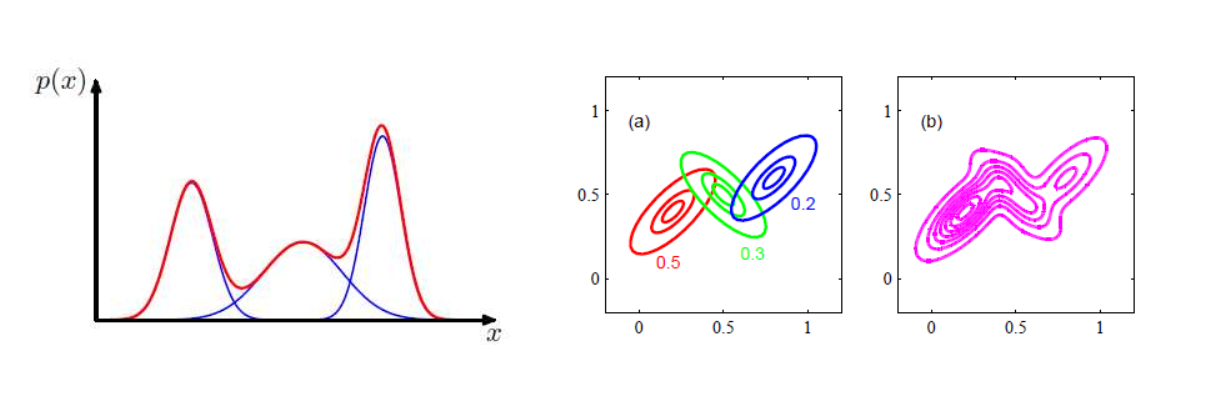
\includegraphics[scale=0.5]{figures/Feature_extraction/FV.png}
	\caption{Bag of words representation}
	\label{FV}
	\end{figure}
	
\end{enumerate}

\section{Summary}
In this chapter we studied about the various feature descriptors that can be used
for videos. We also studied the feature encoding methods and how they are evaluated. In the next chapter, we will look at the various classifiers that we can use dor the purpose of classifying videos.

\chapter{Classifiers}\label{Classifiers}
\thispagestyle{empty}
\setlength{\parskip}{10pt plus 5pt minus 3pt}
\setlength{\parindent}{20pt}%
%
%\documentclass[10pt,a4paper]{article}
%\usepackage[utf8]{inputenc}
%\usepackage[english]{babel}
%\usepackage{amsmath}
%\usepackage{amsfonts}
%\usepackage{amssymb}
%\usepackage{makeidx}
%\usepackage{graphicx}
%\author{Rupali Bhatnagar}
%\begin{document}
\section{GMM}
A Gaussian Mixture Model (GMM) is a parametric probability density function represented as a weighted sum of Gaussian components as seen in Figure \ref{GMM}.\citet{GMM_tut} GMMs are commonly used as a parametric model of the probability distribution of continuous features. GMM parameters are estimated from training data using the iterative Expectation-Maximization (EM) algorithm or Maximum APosteriori (MAP) estimation from a well-trained prior model.\\
A Gaussian mixture model is a weighted sum of M component Gaussian distributions and is represented as:-
\begin{equation}
\mathit{p}\left(x\mid\lambda\right) = \sum_{i=1}^{M}w_i \mathcal{N}\left(x\mid\mu_i\Sigma_i\right)
\end{equation}
where x is a D-dimensional vector and $w_i$ are the mixture weights, where ,
\begin{equation}
\mathcal{N}\left(x\mid\mu_i\Sigma_i\right)=\frac{1}{2\left(\Pi\right)^{\frac{D}{2}} \mid\sigma\mid^{frac{1}{2}}}exp frac{-1}{2}\left(x- \mu_i\right)'\sigma^{-1}_i\left(x-\mu_i\right)
\end{equation}
The mixture weights satisfy the constraint that-
\[ \sum_{i=1}^{M}w_i=1 \]

\begin{figure}[!hbtp]
\centering
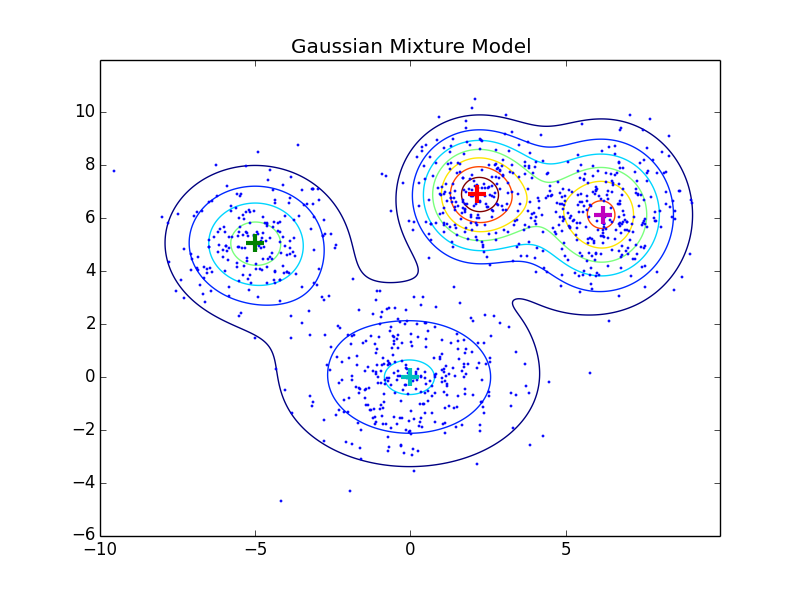
\includegraphics[scale=0.5]{figures/Classifiers/GMM.png}
\caption{Gaussian mixture model}
\label{GMM}
\end{figure}
A GMM is capable of modeling continuous features but is incapable of handling sequence information.
\section{HMM}
An HMM(Hidden Markov Model) is a parametric model which are like finite state automata with continuous or discrete valued observations.An HMM $\lambda$ is defined as \[\lambda=A,B,\Pi\]
where,\\
$A$= state transition probabilities\\
$B$=observation probability matrix\\
$\Pi$=initial state distribution\\

\subsection{The 3 Problems of HMM}\Mycite{Rabiner}

Given a sequence $X=\left( x_0,x_1,x_2,x_3 \ldots \right)$ with corresponding observations $\mathcal{O}=\left(\mathcal{O}_0,\mathcal{O}_1,\mathcal{O}_2,\mathcal{O}_3 \ldots\right)$, the 3 problems of HMM are:-
\begin{enumerate}
\item Given the model  $\lambda=A,B,\Pi$ and a sequence of observations $\mathcal{O}$, find $P\left(\mathcal{O}\mid\lambda\right)$. Here, we
want to determine the likelihood of the observed sequence $\mathcal{O}$, given the model. Use of Forward Backward technique solves this problem.
\item Given $\lambda=A,B,\Pi$ and an observation sequence $\mathcal{O}$, find an optimal state sequence that resulted in generation of $\mathcal{O}$. Use of Baum Welch algorithm solves this problem.
\item Given an observation sequence $\mathcal{O}$ and the dimensions N and M, find the model $\lambda=A,B,\Pi$ that maximizes the probability of O. Use of Viterbi decoding methodology solves this problem.
\end{enumerate}

\begin{figure}[!hbtp]
\centering
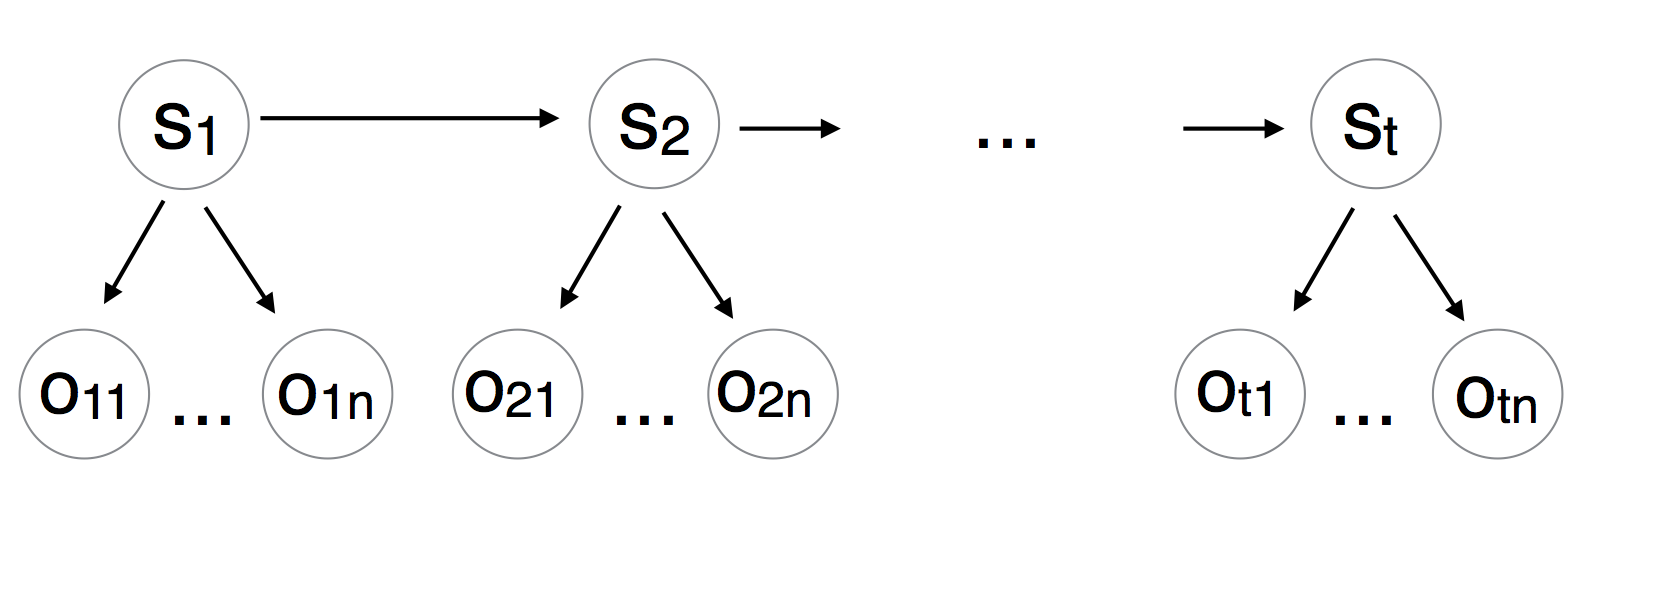
\includegraphics[scale=0.5]{figures/Classifiers/HMM.png}
\caption{Hidden markov model}
\label{HMM}
\end{figure}

\newpage
\section{Support Vector Machines}
Support vector machines are binary classifiers that can classify the data given its features. They work on the principle of Structural Risk Minimization that is based on the statistical learning theory of Vapnik \Mycite{Vapnik_SLT}.SVM is one of the most popular and efficient methods for the task of classification. The detailed description of the working of SVM is presented.


\subsection{Maximum Margin Hyperplane}
In case of linearly separable data, it is easy to construct a separating maximum margin hyperplane between the classes using an SVM.
\begin{figure}[!hbtp]
\centering
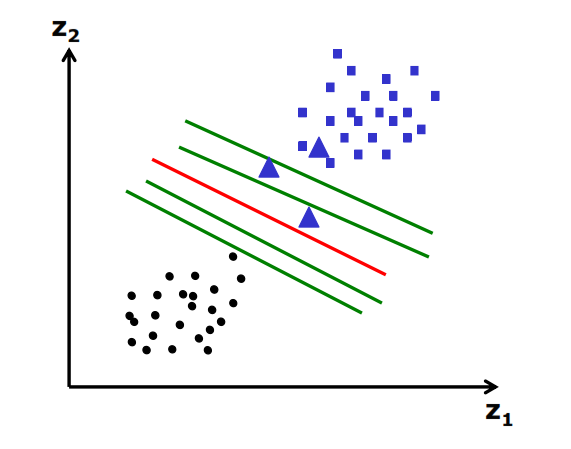
\includegraphics[scale=0.5]{figures/Chapter2/LSD.png}
\caption{Linearly Separable Data\Mycite{Mams_Book}}
\end{figure}

The \textit{margin of a hyperplane} is defined as the minimum distance of training points from the hyperplane.\Mycite{Mams_Book} The SVM tries to create a maximum margin hyperplane, that is, the margin between each class to the hyperplane is maximum.\\
Suppose the training data set consists of L examples,$\lbrace x_i,y_i \rbrace_{i=1}^l, x_i \in R^d$ \& $y_i \in \lbrace +1,-1\rbrace$ where, $x_i$ is $i^{th}$ training example and $y_i$  is the corresponding class label.
A hyperplane is specified as $\boldsymbol{w^tx}+b=0$ where $\boldsymbol{w}$ is the parameter vector and $b$ is the bias. A separating hyperplane that separates the data points of two linearly separable classes satisfies the following constraints:
\begin{equation}
y_i( \boldsymbol{w^tx_i} + b) < 0 \quad \textrm{for} \quad i = 1, 2,...., L 
\end{equation}
The distance between the nearest example and the separating hyperplane, called the margin, is given by $1/||\boldsymbol{w}||$. The problem of finding the optimal separating hyperplane that maximizes the margin is the same as the problem of minimizing the Euclidean norm of the parameter vector $\boldsymbol{w}$. For reducing the search space of $\boldsymbol{w}$, the constraints that the optimal separating hyperplane must satisfy are specified as follows:
\begin{equation}\label{eq2}
y_i( \boldsymbol{w^tx_i} + b) \geq 1 \quad \textrm{for} \quad i = 1, 2,...., L 
\end{equation}

The learning problem of finding the optimal separating hyperplane is a constrained optimization problem stated as follows: Given the training data set, find the values of $\boldsymbol{w}$ and $b$ such that they satisfy the constraints in (\ref{eq2}) and the parameter vector \textbf{w} minimizes the following cost function:
\begin{equation}
J (\boldsymbol{w})=\frac{1}{2} \Vert \boldsymbol{w}^2 \Vert
 \end{equation}
The constrained optimization problem is solved using the method of Lagrangian multipliers. The primal form of the Lagrangian objective function is given by
\begin{equation}\label{Primal}
\L_p{\boldsymbol{w},b,\alpha} = \frac{1}{2}\Vert \boldsymbol(w) \vert^2 - \sum_{i=1}^l\alpha_i[y_i( \boldsymbol{w^tx_i} + b) -1]
\end{equation}

where the non-negative variables $\alpha$  are called Lagrange multipliers. The saddle point of the Lagrangian objective function provides the solution for the optimization problem. The solution is determined by first minimizing the Lagrangian objective function with respect to $\boldsymbol{w}$ and $b$, and then maximizing with respect to $\alpha$. The two conditions of optimality due to minimization are :
\begin{equation}
\frac{\partial \L_p({\boldsymbol{w},b,\alpha})}{\partial \boldsymbol{w}} =0
\end{equation}
\begin{equation}
\frac{\partial \L_p({\boldsymbol{w},b,\alpha})}{\partial b} =0
\end{equation}
Application of optimality condition gives:-
\begin{equation}\label{opt1}
\boldsymbol{w}=\sum_{i=1}^L \alpha_i y_i \boldsymbol{x}_i
\end{equation}
\begin{equation}\label{opt2}
\sum_{i=1}^L \alpha_i y_i =0
\end{equation}

Substituting the expression for $\boldsymbol{w}$ from (\ref{opt1}) in (\ref{Primal}) and using the condition in (\ref{opt2}), the dual form of Lagrangian objective function can be derived as a function of Lagrangian multipliers $\alpha$, as follows:
\begin{equation}\label{Dual}
\L_d(\alpha) =  \sum_{i=1}^l\alpha_i - \frac{1}{2}\sum_{i=1}^L \sum_{j=1}^L\alpha_i\ \alpha_j y_i y_j \boldsymbol{x}_i \boldsymbol{x}_j
\end{equation}
The optimum values of Lagrangian multipliers are determined by maximizing the objective
function $\L_d(\alpha)$ subject to the following constraints:
\begin{equation}
\sum_{i=1}^L \alpha_i y_i =0 \quad ,\alpha_i \geq 0 \quad for \quad i=1,2 \cdots L 
\end{equation}
This optimization problem is solved using quadratic programming methods The data points for which the values of the optimum Lagrange multipliers are not zero are the \textbf{support vectors}. For these data points the distance to the optimal hyperplane is minimum. Hence, the support vectors are the training data points that lie on the margin.
\begin{figure}[!hbtp]
\centering
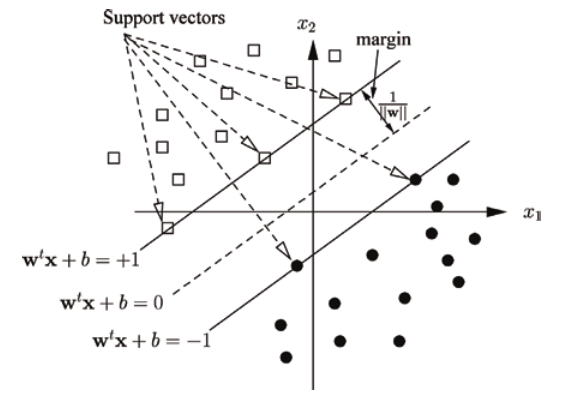
\includegraphics[scale=0.6]{figures/Chapter2/SV_LSD.png}
\caption{Support Vectors for Linearly Separable Data\Mycite{Mams_Book}}
\end{figure}

For the optimum Lagrange multipliers,$\lbrace\alpha^*_j\rbrace_{j=1}^L$, the optimum parameter vector $\boldsymbol{w^*}$ is given by 
\begin{equation}
\boldsymbol{w^*}=\sum_{j=1}^L \alpha_j^* y_j \boldsymbol{x}_j
\end{equation}
where $L_s$ is the number of support vectors. The discriminant function of the optimal hyperplane in terms of support vectors is given by-
\begin{equation}\label{SVK}
\boldsymbol{D}(\boldsymbol{x})=\boldsymbol{w}^{*t}\boldsymbol{x}+b^* =\sum_{j=1}^L \alpha^*_j y_j \boldsymbol{x}^t \boldsymbol{x}_j + b^*
\end{equation}
where $b^*$  is the optimum bias. However, the data for most of the real world  tasks are not linearly separable. 
\subsection{Soft Margin Hyperplane}
For linearly non-separable data, there are a few points that are \textbf{outliers}.That means if we were to create a separating hyperplane, the optimal hyperplane would have a \textit{narrow margin}. For the purpose of generalization, it is better to have a wide margin than having narrow margin. But if we were to have a wide margin, this would imply that the outliers would be misclassified and wold cause error. In such cases,it is desirable to find an optimal hyperplane that minimizes the probability of classification error for the training data set.\Mycite{Mams_Book} A data point is non-separable when it does not satisfy the
constraint in (\ref{eq2}).This corresponds to a data point that falls either within margin or on the wrong side of the separating hyperplane as illustrated.
\begin{figure}[!hbtp]
\centering
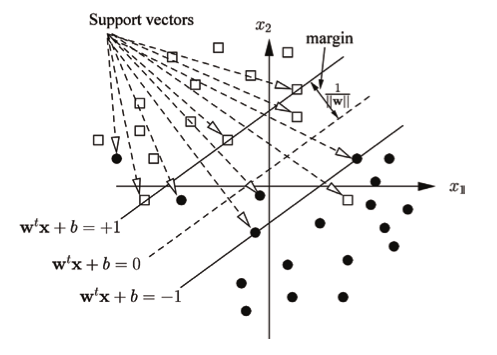
\includegraphics[scale=0.75]{figures/Chapter2/SV_LNSD.png}
\caption{Support Vectors for Linearly Non-Separable Data \Mycite{Mams_Book}}
\end{figure}
For linearly non-separable classes, the constraints in (\ref{eq2}) are modified by introducing the non negative slack variables $\xi_i$ as follows:
\begin{equation}\label{eq2_n}
y_i( \boldsymbol{w^tx_i} + b) \geq 1-\xi_i \quad \textrm{for} \quad i = 1, 2,...., L 
\end{equation}
The slack variable $\xi_i$  is a measure of the deviation of a data point $\boldsymbol{x}_i$ from the ideal condition of separability. For $0 \leq \xi_i  \leq 1$, the data point falls inside the region of separation, but on the correct side of the separating hyperplane. For, $\xi_i >1 $ the data point falls on the wrong side of the separating 
hyperplane. The support vectors are those particular data points that satisfy the constraint in (\ref{eq2_n}) with equality sign. The cost function for linearly non-separable classes is given as-
\begin{equation}
J (\boldsymbol{w},\boldsymbol{\xi})=\frac{1}{2} \Vert \boldsymbol{w}^2 \Vert +C \sum_{i=1}^L\xi_i
 \end{equation}
where C is a user-specified positive parameter that controls the trade-off between the complexity of the classifier and the number of non-separable data points. Using the method of Lagrange multipliers to solve the constrained optimization problem as in the case of linearly separable classes, the dual form of the Lagrangian objective function can be
obtained as follows:
\begin{equation}\label{Dual_n}
\L_d(\alpha) =  \sum_{i=1}^l\alpha_i - \frac{1}{2}\sum_{i=1}^L \sum_{j=1}^L\alpha_i\ \alpha_j y_i y_j \boldsymbol{x}_i^t \boldsymbol{x}_j
\end{equation}
subject to the constraints:-
\begin{equation}
\sum_{i=1}^L \alpha_i y_i =0 \quad ,\alpha_i \geq 0 \quad for \quad i=1,2 \cdots L 
\end{equation}
It may be noted that the maximum value that the Lagrangian multipliers $\alpha_i$  can take is $C$ for the linearly non-separable classes. For the optimum Lagrange multipliers
$\lbrace\alpha^*_j\rbrace_{j=1}^L$ ,the optimum parameter vector $\boldsymbol{w^*}$ is given by 
\begin{equation}
\boldsymbol{w^*}=\sum_{j=1}^L \alpha_j^* y_j \boldsymbol{x}_j
\end{equation}
where $L_s$ is the number of support vectors.The discriminant function of the optimal hyperplane in terms of support vectors is given by-
\begin{equation}\label{SVK_n}
\boldsymbol{D}(\boldsymbol{x})=\boldsymbol{w}^{*t}\boldsymbol{x}+b^* =\sum_{j=1}^L \alpha^*_j y_j \boldsymbol{x}^t \boldsymbol{x}_j + b^*
\end{equation}
where $b^*$  is the optimum bias.

\subsection{Kernel based SVM}
It is easy to create SVM for linearly separable data and linearly non-separable data. But for non-linearly separable data \& overlapping data, we cannot use directly use the above strategies since the data is not linearly separable. So, for non-linearly separable classes, an SVM is built by mapping the input vector $\boldsymbol{x}_i$, i = 1, 2, …, L into a high dimensional feature vector $\boldsymbol{\phi}({\boldsymbol{x}}_i)$ using a nonlinear transformation $\boldsymbol{\phi}$, and constructing an optimal hyperplane defined by $\boldsymbol{w^t\phi(x)}+b=0$ to separate the examples of two classes in the feature space . This is based on the Cover's Theorem-
\begin{theorem}[Cover's Theorem]
A complex pattern-classification problem, cast in a high-dimensional space non-linearly, is more likely to be linearly separable than in a low-dimensional space, provided that the space is not densely populated.
\end{theorem}
\begin{figure}[!hbtp]
\centering
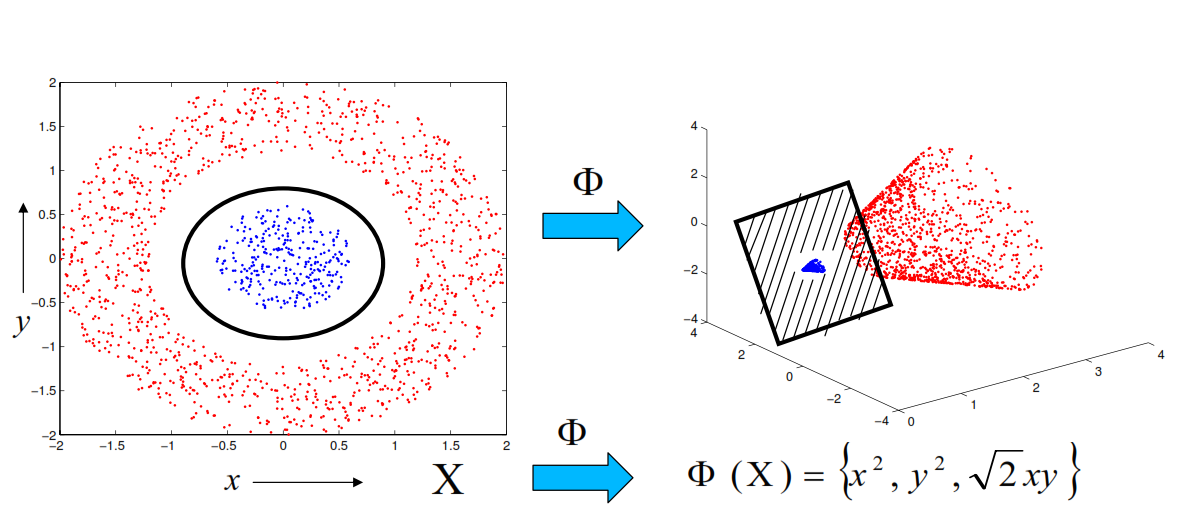
\includegraphics[scale=0.5]{figures/Chapter2/Kernel_trans.png}
\caption{Kernel transformation for non-linearly separable data}
\end{figure}
For the construction of the optimal hyperplane in the high dimensional feature space $\boldsymbol{\phi}({\boldsymbol{x})}$, the dual form of the Lagrangian objective function in (\ref{Dual_n}) takes the following form:
\begin{equation}\label{Dual_kernel}
\L_d(\alpha) =  \sum_{i=1}^l\alpha_i - \frac{1}{2}\sum_{i=1}^L \sum_{j=1}^L\alpha_i\ \alpha_j y_i y_j \boldsymbol{\phi}({\boldsymbol{x}}_i)^t \boldsymbol{\phi}({\boldsymbol{x}}_i)
\end{equation}
subject to the constraints-
\begin{equation}
\sum_{i=1}^L \alpha_i y_i =0 \quad ,0 \leq \alpha_i \leq C \quad for \quad i=1,2 \cdots L 
\end{equation}
For the optimum Lagrange multipliers$\alpha^*$ ,the optimal vector $\boldsymbol{w^*}$ is given by 
\begin{equation}
\boldsymbol{w^*}=\sum_{j=1}^L \alpha_j^* y_j  \boldsymbol{\phi}({\boldsymbol{x}}_j)
\end{equation}
where $L_s$ is the number of support vectors.The discriminant function of the optimal hyperplane for an input vector x is defined as-
\begin{equation}\label{SVK_kernel}
\boldsymbol{D}(\boldsymbol{x})=\boldsymbol{w}^{*t|}_|(\boldsymbol{x})+b^* =\sum_{j=1}^L \alpha^*_j y_{j|}^| (\boldsymbol{x})^{t|}_| \boldsymbol{x}_j + b^*
\end{equation}
where $b^*$  is the optimum bias.Solving (\ref{Dual_kernel}) involves computation of the inner product operation $\boldsymbol{\phi}({\boldsymbol{x}}_j)^t \boldsymbol{\phi}(\boldsymbol{x}_j)$. Evaluation of inner products in a high dimensional feature space
is avoided by using an inner product kernel, $K(\boldsymbol{x}_i,\boldsymbol{x}_j)$, defined as $K(\boldsymbol{x}_i,\boldsymbol{x}_j)=\boldsymbol{\phi}(\boldsymbol{x}_i)^t\boldsymbol{\phi}(\boldsymbol{x}_j)$.A valid innerproduct kernel $K(\boldsymbol{x}_i,\boldsymbol{x}_j)$ for two pattern vectors $\boldsymbol{x}_i$ and $\boldsymbol{x}_j$ is a symmetric  function for which the following Mercer’s condition holds good:
\begin{theorem}[Mercer's Condition]
A real-valued function $K(x,y)$ is said to fulfill Mercer's condition if for all square integrable functions $g(x)$ one has-
\begin{equation}
\int \int K(\boldsymbol{x}_i,\boldsymbol{x}_j)g(\boldsymbol{x}_i)g(\boldsymbol{x}_j)d\boldsymbol{x}_i d\boldsymbol{x}_j \geq 0
\end{equation}
for all $g(\boldsymbol{x}_i)$ such that
\begin{equation}
g^2(\boldsymbol{x}_i)d\boldsymbol{x}_i < \infty
\end{equation}
\end{theorem}
The architecture of a support vector machine for two-class pattern classification that implements the discriminant function of the hyperplane is given. The number of hidden nodes 
corresponding to the number of support vectors, and the training examples corresponding to the support vectors are determined by maximizing the objective function using a given training data set and for a chosen kernel function.

\begin{figure}[!hbtp]
\centering
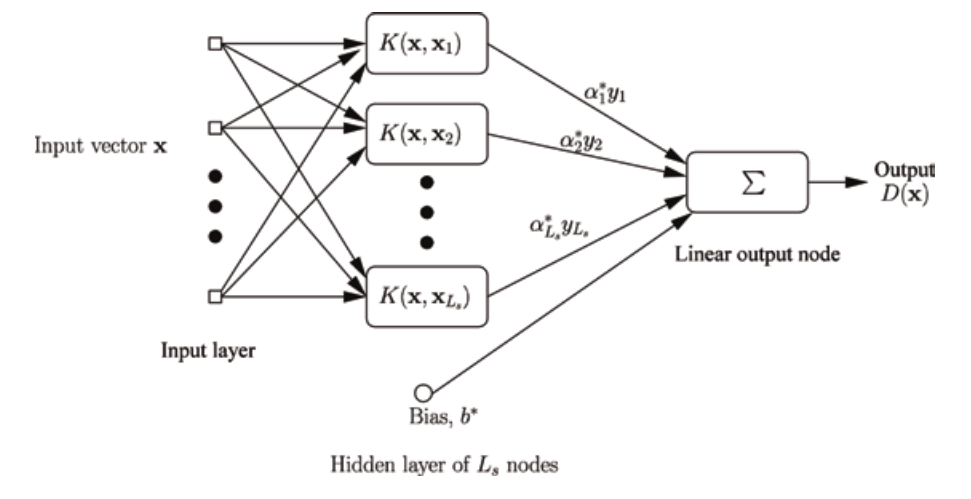
\includegraphics[scale=0.6]{figures/Chapter2/SVM.png}
\caption{Architecure of SVM \Mycite{Mams_Book}}
\end{figure}


Some commonly used inner product kernel
functions are as follows:\\
\textbf{Polynomial kernel}:$K(\boldsymbol{x}_i,\boldsymbol{x}_j)=(a\boldsymbol{x}_i^t\boldsymbol{x}_j+c)^p$ \\
\textbf{Sigmoidal kernel}: $K(\boldsymbol{x}_i,\boldsymbol{x}_j)=tanh(\boldsymbol{x}_i^t\boldsymbol{x}_j+c)$\\
\textbf{Gaussian kernel}: $K(\boldsymbol{x}_i,\boldsymbol{x}_j)=\exp{-\delta\Vert\boldsymbol{x}_i-\boldsymbol{x}_j\Vert^2}$

\subsection{Kernel Methods for SVM}
For the task of sequential pattern classification, there are 2 types of approaches used:-
\begin{enumerate}
\item Hybrid SVM/HMM based approach- In this approach, the varying length pattern is first mapped to a fixed length and then a kernel for fixed length patterns is used for classification. The result of the SVM classification is then used as posterior probability for computing the log likelihood probability in the HMM.
\item Dynamic Kernel based approach-In this approach, a suitable kernel for varying length patterns, called dynamic kernels, is designed. 
\end{enumerate}

%%%%%%%%%%%%%%%%%%%%%%%%%%%%%%%%%%%%%%%%%%%%%%%%%%%%%%%%%%%%%%%%%%%%%%%%%%%%%%%%%
\section{Dynamic Kernels}
Dynamic kernels are kernels designed for classification of varying length input patterns through SVM. There are various approaches to design dynamic kernels.

\subsection{Explicit Mapping based Approaches}-
Explicit Mapping based approaches involve mapping a sequence feature vector into a fixed dimensional representation and then defining a kernel function in the space of that representation.They include:-
\begin{enumerate}
\item Fisher Kernel
\item Likelihood Ratio Kernel
\end{enumerate}
They are computationally intensive to calculate because they use an HMM for mapping the sequence into a fixed dimensional Fisher score-space in which the kernel is computed.


\subsection{Probabilistic distance based Approaches}-
In the probabilistic distance based approach,a suitable distance measure between the probability distributions corresponding to the two sequences of
feature vectors is used as the kernel.

The probability product kernel is an example of this approach. In the probability product kernel, each sequence is represented by an HMM and the kernel is obtained by kernelizing the Kullback-Liebler divergence
\footnote{Kullback-Liebler divergence or KL divergence is the measure of difference between 2 probability distributions P \& Q, where P represents the ``true'' distribution or the theoretical distribution while Q calculates the ``model'' or experimentaional approximation of P.
\begin{center}
$D_{KL}(P \Vert Q)=\Sigma{_i} P(i) \log{\frac{P(i)}{Q(i)}}$
\end{center}
}
between the 2 HMM's.

\subsection{Mapping Based Approaches}
The mapping based approaches, also known as alignment kernels compute kernel between a pair of sequences in a parametric vector space using Dynamic Time Warping (DTW) kernel. They include the following methodologies:-
\begin{enumerate}
\item Dynamic Time Warping kernel
\item Dynamic Time Alignment kernel
\item Global Alignment kernel
\item Triangular Global alignment kernel
\item Intermediate matching kernel
\end{enumerate} 

\subsubsection{Intermediate Matching Kernel}
Intermediate Matching kernel is a mapping based approach in which the kernel between the 2 sets of feature vectors is created by mapping the varying local feature vectors into fixed length virtual feature vectors and then computing a kernel using the set of virtual feature vectors. Various intermediate matching kernels are present in literature:- 
\begin{enumerate}
\item GMM-IMK- Proposed by \citet{GMMIMK},the GMM-IMK is constructed by making a GMM over all the training data. Then the GMMIMK is computed as the the sum of values of the base kernel computed for each of the 'Q' pairs of selected local feature vectors , where Q= number of components of the constructed GMM. The GMM-IMK does not capture the sequence information and therefore is not suitable for classification of videos.
\item HMM-IMK-Proposed by \citet{HIMK}, the HIMK is constructed by making a continuous density HMM for each class using the training data for that particular class.We discuss HIMK in detail in Chapter \ref{Proposed_approach}.
\end{enumerate}

\section{Summary}
In this chapter, we discussed about the various classifier methodologies present in the literature. We rationalized whether the methodology could be used for the purpose of classification of videos or not. We now present our approach for video classification.
%\end{document}

\chapter{Proposed Approach}\label{Proposed_Approach}
\thispagestyle{empty}
\setlength{\parskip}{10pt plus 5pt minus 3pt}
\setlength{\parindent}{20pt}%

%\documentclass[10pt,a4paper,oneside]{article}
%\usepackage[utf8]{inputenc}
%\usepackage[english]{babel}
%
%\usepackage{amsfonts}
%\usepackage{amssymb}
%\usepackage{makeidx}
%\usepackage{graphicx}
%\usepackage{amsmath}
%\usepackage{algorithm}
%
%\usepackage[noend]{algpseudocode}
%\algnewcommand{\Inputs}[1]{%
%  \State \textbf{Inputs:}
%  \Statex \hspace*{\algorithmicindent}\parbox[t]{.8\linewidth}{\raggedright #1}
%}
%\algnewcommand{\Initialize}[1]{%
%  \State \textbf{Initialize:}
%  \Statex \hspace*{\algorithmicindent}\parbox[t]{.8\linewidth}{\raggedright #1}
%}
%
%\usepackage{mathtools} % Bonus
%\newtheorem{theorem}{Theorem}
%
%\DeclareMathOperator*{\argmax}{arg\,max}
%
%
%\author{Rupali Bhatnagar}
%\begin{document}


For classifying actions, we use the following methodology:-
\begin{enumerate}
\item Feature Extraction
\item Evaluation of Kernel
\item Classification using SVM and evaluated kernel
\end{enumerate}


\section{Feature Extraction}

\subsection{Histogram of Oriented Gradient Features}
For the task of feature extraction, we use Histogram of Oriented Gradients(HoG). We use \citet{HOG} methodology to extract set features for each frame of the video. These set features are then appended to created HoG set feature vector. \\
This can be easily visualized in the \figurename{~\ref{fig:HoG}}.

\begin{figure}[!hbtp]
\centering
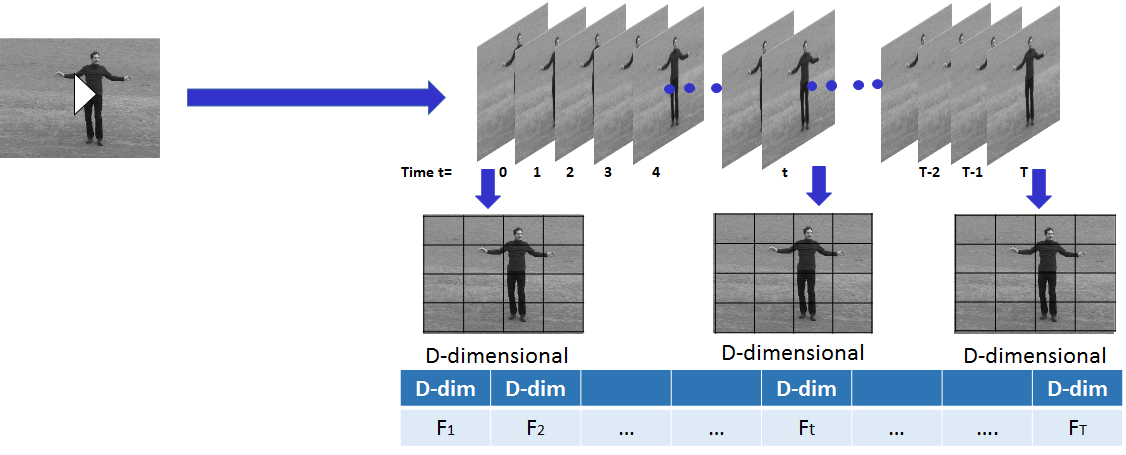
\includegraphics[scale=0.5]{figures/Proposed_Approach/Feature_Extraction.png}
\caption{Histogram of oriented gradients feature extraction from video}
\label{fig:HoG}
\end{figure}
\newpage
In \figurename{~\ref{fig:HoG}}, the video is divided into constituent frames. The frame is further subdivided into sets. The HoG feature of each set is then taken and appended to get a D-dimensional feature vector of each frame .\\

If there are `f' frames in the video, then the representation of one video would be of order O(fD). This results in a dense representation for the video dataset which is in very huge in size.


\subsection{Bag of Visual Words model}
The Bag Of Visual Words(BoVW) is an extension of the Bag of Words model that is used for document classification.The bag of visual words model is present for images. For videos, it is extended as follows:-
\begin{enumerate}
\item Feature Detection- The set features extracted using HoG feature descriptor is used to detect objects in the frames.The frame feature is a concatenation of HoG features extracted from each set. The video features is a concatenation of the frame features that we obtain previously.\\

\item Codebook Generation- To get the visual words, we cluster the whole data using a suitable clustering mechanism. Since each feature in the video feature representation is a histogram, it is better to use a distance measure that captures the similarity between histograms.The process of codebook generation can be visualized in the Figure \ref{codebook}\\

\begin{figure}[!hbtp]
\centering
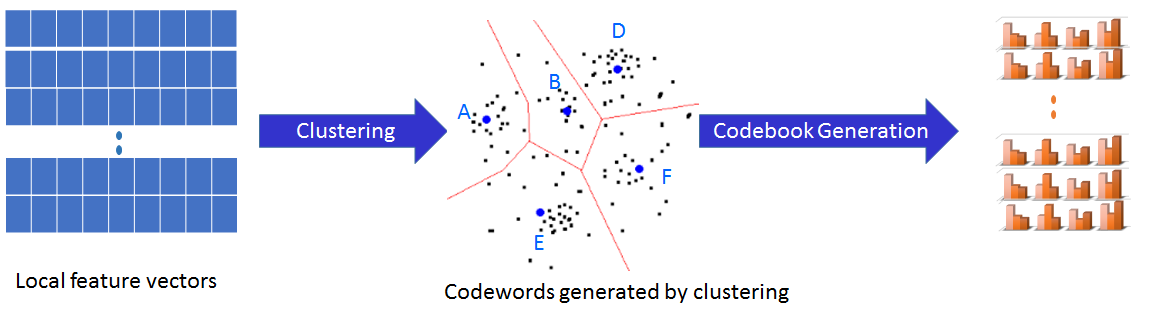
\includegraphics[scale=0.5]{figures/Proposed_Approach/Codebook_Generation.png}
\caption{Codebook generation for feature extraction}
\label{codebook}
\end{figure}

We use the Histogram Match Score as given by Algorithm \ref{HistScore} for measuring the similarity between the 2 histograms. The Histogram Match score based K-medoid algorithm is defined in Algorithm \ref{Kmedoid}\\

\begin{algorithm}[H]
\caption{Histogram Matching Score }
\label{HistScore}
\begin{algorithmic}
\Inputs{Histogram vectors $h_{i}$ and $h_{j}$}
\Initialize{score $\gets 0$}
\For{i :=0 $\to$ num\_bins}
	\State score $\gets$ score + $\min$($h_i(i),h_{j}(i)$)
\EndFor

	\State score $\gets \frac{score}{num_bins}$
	\State return score\;

\end{algorithmic}
\end{algorithm}


\begin{algorithm}[H]
\caption{Histogram Matching Score based -  K-medoid algorithm}
\label{Kmedoid}
\begin{algorithmic}[1]
\Inputs{k := number of clusters}
\Initialize{$\lbrace x_{1} , x_{2} \ldots x_{k}\rbrace \gets$ k random cluster centers}
\While{$\lbrace x_{1} , x_{2} \ldots x_{k}\rbrace$ 	not converged }
	\For{each data vector $v_{i}$}
		\For{each cluster center $x_{k}$}
    		\State Calculate Histogram Matching Score between $v_{i}$ and $x_{k}$
		\EndFor
		\State For the data vector $v_{i}$ assign index as:
		\State index($v_{i}$)$\gets$ $\max$(Histogram Matching Score w.r.t all the cluster centers)
    \EndFor
    
 	\For{each cluster k}
 		\State New cluster center $x_{k}$ = medoid of all the Histogram Scores in the cluster
 	\EndFor
 	
 	\For{each k}
 		\If {$x_{new}$ == $x$}
 			\State return Converged
 		\Else
 			\State return Not Converged
 		\EndIf
 	\EndFor
 \EndWhile		

\end{algorithmic}
\end{algorithm}

\end{enumerate}

\section{Evaluation of Kernel}
After the feature extraction phase, we get a set feature vector representation for a video. A video with T frames is represented as a sequential pattern $X=\lbrace x_1,x_2, \ldots x_T\rbrace$, where $x_t$ is the feature vector for a frame at time $t$.Since the number of frames depends on the duration of the video, the length of the pattern representing different videos would be different.\\
Hidden Markov Models(HMM) are usually used for classifying sequences of feature vectors.Since the symbols in the set of feature vector is not discrete, we use continuous density HMM (CDHMM) in our proposed approach.

\subsection{HMM based Intermediate Matching Kernel}
HMM based Intermediate Matching Kernel(HIMK) is a dynamic kernel which is constructed by matching local feature vectors in the 2 feature vectors with the help of virtual feature vectors.The HIMK is therefore constructed by using a continuous density HMM (CDHMM. \citet{HIMK} have designed 2 methods of creating HIMK.\\

In the first approach, they create HIMK by using \textit{subsequence matching} where the subsequences are aligned with the optimal state sequence obtained by using Viterbi's method. Then, a GMM-based IMK for the subsequence aligned at a particular state of the HMM is constructed using the GMM of that state to get the virtual feature vectors. \\

In the second approach, the HIMK is created using \textit{complete sequence matching} in which the virtual feature vectors are selected using the responsibility term of all the components of the GMM at each state of the HMM without and then summing the base kernel over these selected virtual feature vectors. 

\begin{figure}[!hbtp]
\centering
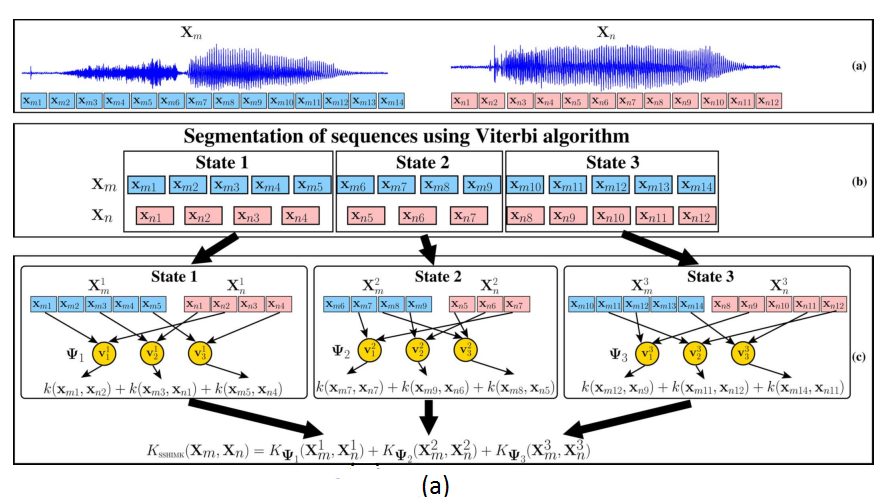
\includegraphics[scale=0.5]{figures/Proposed_Approach/Subsequence_HIMK.png} 
\caption{(a)HIMK created using subsequence matching\Mycite{HIMK}}
\end{figure}

\begin{figure}[!hbtp]
\centering
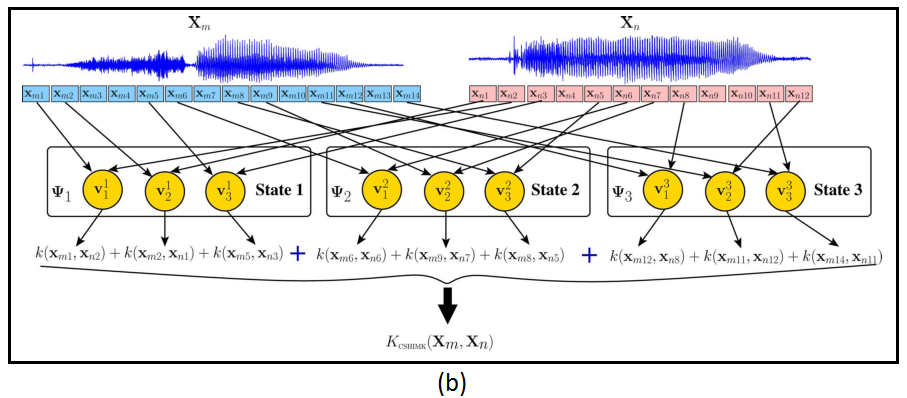
\includegraphics[scale=0.6]{figures/Proposed_Approach/CompleteSequence_HIMK.png} 
\caption{(b)HIMK created using complete sequence matching \Mycite{HIMK}}
\end{figure}

We use the complete sequence matching based HIMK for our work.

\subsection{Complete Sequence Matching based HIMK}
For 2 videos, $X_m=\lbrace x_m1,x_m2, \ldots x_{m{T_m}}\rbrace$ and $X_n=\lbrace x_n1,x_n2, \ldots x_{n{T_n}}\rbrace$, the virtual feature vectors for the $q^th$ component of GMM of the $i^th$ state of the HMM are defined as:-

\begin{equation}
x^{*}_{miq}= \argmax_{x_t \in X_m}\mathit{R_{iq}}\left( x_t \mid \mathbf{X}_m,\lambda\right)
\end{equation}
 and  
 \begin{equation}
x^{*}_{niq}= \argmax_{x_t \in X_n}\mathit{R_{iq}}\left( x_t \mid \mathbf{X}_n,\lambda\right)
 \end{equation}

where,
\\ for the continuous density HMM $\lambda$, the probability of being in state $\mathit{i}$ at time $\mathit{t}$ and the $\mathit{q}^{th}$ component of GMM $\Psi_\mathit{i}$ of state $\mathit{i}$ for the local feature $x_t$ in the sequence $\mathbf{X}$ is given by:-

\begin{equation}
\mathit{R}_{iq}\left(x_t \mid \mathbf{X},\lambda\right)=\nu_{it}\gamma_{iq}\left(x_t\right)
\end{equation}

Here,$\nu_{it}$ is the probability of being in state $\mathit{i}$ at time $\mathit{t}$ and given $\mathbf{X}$ and $\lambda$,
\begin{equation}
\nu_{it}= \mathit{P}\left[s_t=\mathit{i} \mid \mathbf{X},\lambda\right] 
\end{equation}

Then, the HIMK is calculated as:-
\begin{equation}
\mathit{K}_{HIMK}\left(\mathbf{X}_m,\mathbf{X}_n\right)=\sum_{i=1}^{N} \sum_{q=1}^{Q_i}\mathit{k}\left(x^*_{miq},x^*_{niq}\right)
\end{equation}
where, $Q_i$ is the number of components of the GMM $\Psi_i$ and $\mathit{k}$ is the base kernel.\begin{figure}[!hbtp]
\centering
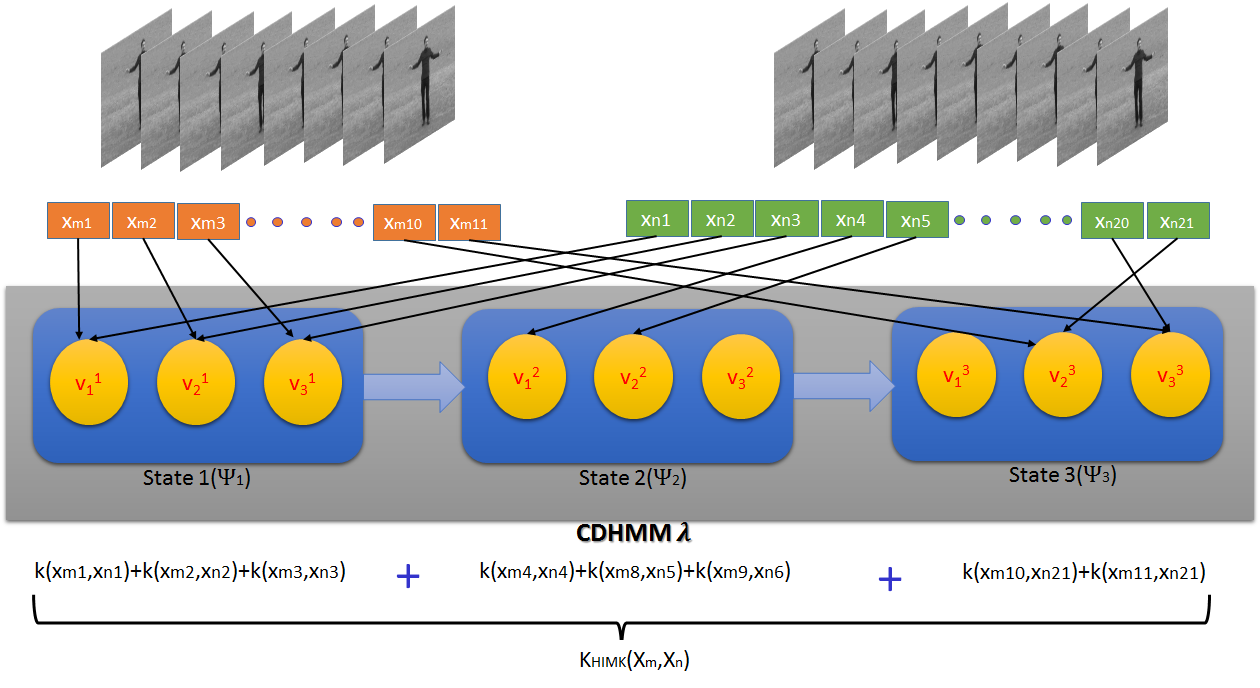
\includegraphics[scale=0.5]{figures/Proposed_Approach/Proposed_HIMK.png}
\caption{Calculation of HMM based Intermediate Matching Kernel}
\end{figure}


\section{Classification using SVM and HIMK}
After getting the HIMK based kernels, we use SVM to classify the test data. SVM uses Kernel Gram Matrices generated using the HIMK for the purpose of classification.

\section{Summary}
In this chapter, we discussed the proposed model and how it works. We studied the HIMK and why is being applied to our data. In the next chapter, we will look at the experimentation results.
%\end{document}
\chapter{Observations and Results}\label{Observations}
\thispagestyle{empty}
\setlength{\parskip}{10pt plus 5pt minus 3pt}
\setlength{\parindent}{20pt}%

%\documentclass[10pt,a4paper]{article}
%\usepackage[utf8]{inputenc}
%\usepackage[english]{babel}
%\usepackage{amsmath}
%\usepackage{amsfonts}
%\usepackage{amssymb}
%\usepackage{makeidx}
%\usepackage{graphicx}
%\author{Rupali Bhatnagar}
%\begin{document}
In the previous chapter, we discussed our proposed model. Our proposed model consisted of 3 stages : feature extraction, HIMK kernel evaluation and SVM classification. We will now discuss the experimental setup and discuss the observations from the experiment results.

\section{Dataset}
The task of classification of human activity recognition, we have use the KTH dataset which consists of trimmed videos for the following 6 types of human action classes:-
\begin{itemize}
\item Boxing
\item Handclapping
\item Handwaving
\item Jogging
\item Running
\item Walking
\end{itemize}
The KTH datset consists of 25 subjects and is pre-divided into the training set, validation set and testing set.The videos are downsampled to the spatial resolution of 160x120 pixels and have a length of four seconds in average.

\section{Results on proposed model}
\subsection{HMM based Intermediate Matching Kernel}
In the proposed system, we create continuous density HMM for the different classes. For each of the class in the dataset,  a continuous density HMM was created with following specifications as per Table \ref{specsHMM}. \\

\begin{table}[!h]
\centering
\begin{tabular}{||c|c|c||}
\hline
Class Label & No of states in CDHMM & No of components of GMM\\
\hline
Boxing&5&3\\
Handclapping&5&3\\
Handwaving&9&3\\
Jogging&20&3\\
Running&20&3\\
Walking&20&3\\
\hline
\end{tabular}
\caption{Specifications for CDHMM of each activity class}
\label{specsHMM}
\end{table}

The HMM states corresponding to the some of the actions can be visualized as in Figure \ref{boxing}, Figure \ref{handclapping} and Figure \ref{handwaving}.

\begin{figure}[!hbtp]
\centering
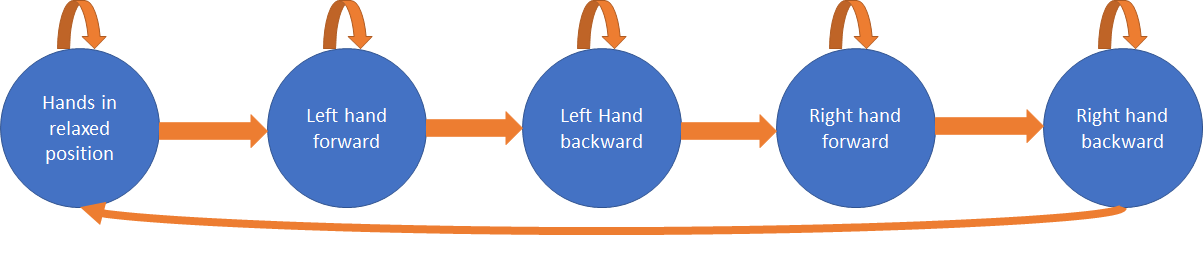
\includegraphics[scale=0.5]{figures/Observations/Boxing.png}
\caption{HMM for boxing class}
\label{boxing}
\end{figure}
\begin{figure}[!hbtp]
\centering
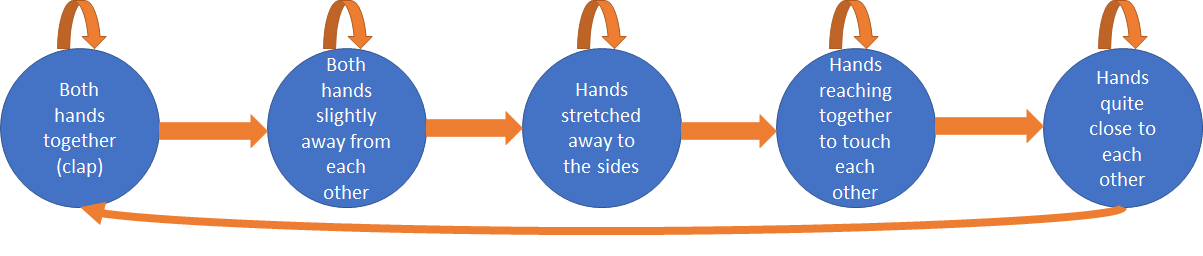
\includegraphics[scale=0.5]{figures/Observations/Handclapping.png} 
\caption{HMM for hand clapping class}
\label{handclapping}
\end{figure}

\begin{figure}[!hbtp]
\centering
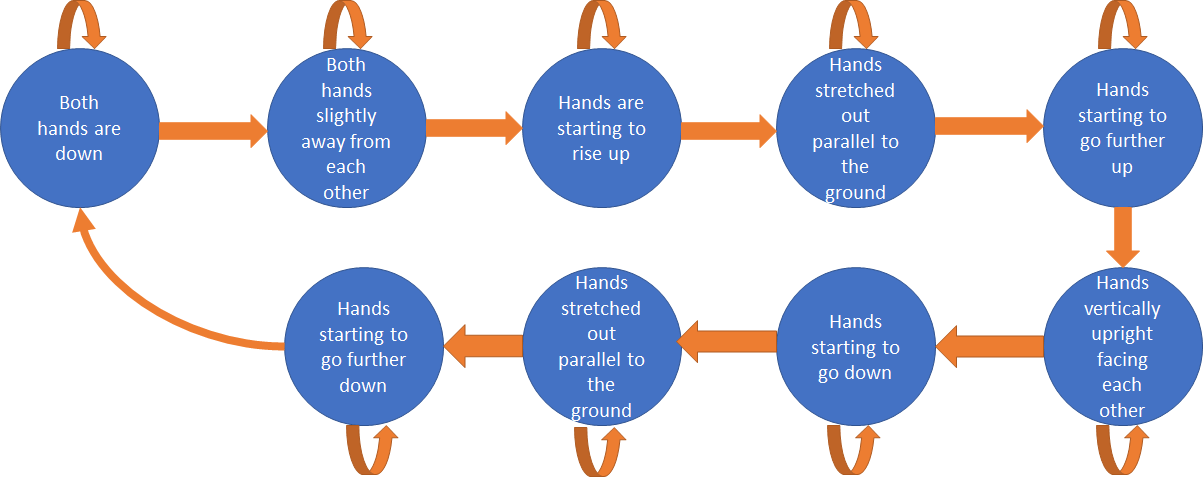
\includegraphics[scale=0.5]{figures/Observations/Handwaving.png} 
\caption{HMM for hand waving class}
\label{handwaving}
\end{figure}

\newpage

\subsection{SVM Classification Results}
For classification using SVM, we used modified version of SVMTorch which allows to specify user defined kernels.The confusion matrix obtained by the proposed methodoly is presented in Table \ref{proposed_CM}
\begin{table}[!htbp]
\centering
\begin{tabular}{|c|c|c|c|c|c|c|}
\hline
 &Boxing&Handclapping&Handwaving&Jogging&Running&Walking\\
 \hline
Boxing&\textbf{63.7\%}&6.72\%&2.61\%&7.34\%&15.9\%&3.73\%\\
Handclapping&11.31\%&\textbf{71.48\%}&8.41\%&2.64\%&5.11\%&1.05\%\\
Handwaving&18.26\%&12.39\%&\textbf{65.34\%}&1.4\%&2.03\%&0.58\%\\
Jogging&8.61\%&1.26\%&1.4\%&\textbf{49.54\%}&22.9\%&16.29\%\\
Running&4.65\%&0.16\%&0.67\%&19.61\%&\textbf{62.18\%}&12.73\%\\
Walking&5.13\%&2.19\%&4.31\%&23.47\%&12.29\%&\textbf{52.61\%}\\
\hline
\end{tabular}
\caption{Percentage wise confusion matrix using Proposed Method}
\label{proposed_CM}
\end{table}

The accuracy of the proposed method comes out to be 60.81\%.

\subsection{Observations}
Looking at the confusion matrix from the Table \ref{proposed_CM}, we can make a few observations :-
\begin{enumerate}
\item For the boxing action class, there seems to be a lot of similarity with the running class. This may be due to the similar movement of hands in both the cases.
\item For the jogging class, the classification result is low because appearance wise, jogging, running and walking are similar and the difference only lies in the speed of movement.
\item For the walking class, the classifier is uncertain as to classify it in jogging class or walking class or running class. This is because the speed of motion is not captured thoroughly by the system.
\end{enumerate}

\section{Results using HMM}
The HMM methodology that was discussed in \ref{HMM}. For training, we pass each example of each class to the HMM created for that class. For testing, we pass the examples to all the trained HMMs and assign the class label for the test example as the class of the HMM that gives the highest posterior probability. Table \ref{HMM_CF}
\begin{table}[!htbp]
\centering
\begin{tabular}{|c|c|c|c|c|c|c|}
\hline
 &Boxing&Handclapping&Handwaving&Jogging&Running&Walking\\
 \hline
Boxing&\textbf{37.9}%&8.3\%&2.61\%&7.34\%&15.9\%&3.73\%\\
Handclapping&11.31\%&\textbf{71.48\%}&8.41\%&2.64\%&5.11\%&1.05\%\\
Handwaving&18.26\%&12.39\%&\textbf{65.34\%}&1.4\%&2.03\%&0.58\%\\
Jogging&8.61\%&1.26\%&1.4\%&\textbf{49.54\%}&22.9\%&16.29\%\\
Running&4.65\%&0.16\%&0.67\%&19.61\%&\textbf{62.18\%}&12.73\%\\
Walking&5.13\%&2.19\%&4.31\%&23.47\%&12.29\%&\textbf{52.61\%}\\
\hline
\end{tabular}
\caption{Percentage wise confusion matrix using HMM}
\label{HMM_CF}
\end{table}


\section{Results using the String kernel}
The string kernel approach for videos was presented by Ballan. In this methodology, they represent each video as a phrase composed of characters. For comparing phrases, they use the concept of \textit{edit distances} using the Needleman-Wunsch edit distance. To compare different characters of the video represented as a phrase, they use the following distance metrics :-
\begin{enumerate}
\item Chi square
\item Kolomogrov -Smirnov
\item Bhattacharya
\item Intersection
\item Correlation
\item Mahalanobis distance
\end{enumerate}

We evaluate results on the dataset using their methodology and get the results as presented in Table \ref{string_CM}

\begin{table}[!htbp]
\centering
\begin{tabular}{|c|c|}
\hline
Distance Metric & Accuracy\\
\hline
\textbf{Chi Square Metric} & \textbf{52.5\%}\\
Kolomogrov Smirnov metric & 48.37\%\\
Bhattacharya distance & 43.56\%\\
Intersection metric & 51.48\%\\
Correlation metric & 47.31\%\\
Mahalanobis distance metric & 37.98\%\\
\hline
\end{tabular}
\caption{Percentage wise confusion matrix using String Kernel}
\label{string_CM}
\end{table}

The highest accuracy for the string kernel methodology comes out to be around 52.5\%

\section{Comparison of the experimental results}
As seen from Table \ref{comparison}, it is easily observed that out proposed approach gives better results than the accuracy achieved through the existing string kernel approach. Though in the literature, work has been done to achieve higher accuracy, the proposed model lies comparable to the newer models as well.
\begin{table}[!htbp]
\centering
\begin{tabular}{|c|c|c|}
\hline
Representation & Accuracy\\
\hline
String kernel with Chi Square Metric & 52.5\%\\
String kernel with Intersection metric & 51.48\%\\
String kernel with Kolomogrov Smirnov metric & 48.37\%\\
String kernel with Correlation metric & 47.31\%\\
\hline
\textbf{Proposed method} &\textbf{ 60.81\%}\\
\hline
\end{tabular}
\caption{Comparison of the accuracy of classification}
\label{comparison}
\end{table}

%\end{document}
\chapter{Conclusion and Future Directions}\label{Conclusion}
\thispagestyle{empty}
\setlength{\parskip}{10pt plus 5pt minus 3pt}
\setlength{\parindent}{20pt}%

\section{Conclusions}
In the previous chapters we learnt the various features and the classifiers that have been used in the area of human activity recognition. We discussed the proposed approach for classifying human actions and discussed the methodology to get the feature representation for videos. Then we looked at the working of the HIMK based SVM classification for video data.\\
We used KTH dataset for experimentation and after looking at the results, we realized that the proposed model works better than the existing string kernel based model. 

\section{Future Work}
Looking at the results in Table \ref{comparison}, it can be easily deduced that the proposed system along with some modifications can be really helpful in the area of human action recognition.\\
We propose the following possible areas where work can be done:-
\begin{enumerate}
\item Use of motion features that capture the velocity of the action can be done.
\item Currently, there has been a shift to the deep learning methodologies for the area of videos. The deep learning based features can be explored for the task of human action recogntion.
\item We can also look at various modifications to the HIMK as proposed by Dileep to get better results.
\end{enumerate}



\appendix
\clearpage

\pdfbookmark{References}{References}
\addcontentsline{toc}{chapter}{References}

%% This defines the bibliography file (main.bib) and the bibliography style.
%% If you want to create a bibliography file by hand, change the contents of
%% this file to a `thebibliography' environment.  For more information 
%% see section 4.3 of the LaTeX manual.
\begin{singlespace}
\phantomsection

\bibliographystyle{plainnat}
%\bibliographystyle{IEEEtran}
\bibliography{references/Bibliography}
\addcontentsline{toc}{chapter}{Bibliography}
\end{singlespace}


\clearpage 
\phantomsection
\normalsize
 \clearpage
\singlespacing
{\small
\phantomsection	
\addcontentsline{toc}{chapter}{Index}}\printindex
\clearpage




\end{document}
